\documentclass[11pt,a4paper]{article}

% ==================================================================
%  Layout and fonts
% ==================================================================
\usepackage[T1]{fontenc}
\usepackage[sc]{mathpazo}
\usepackage[margin=1in,headheight=14pt]{geometry}
\usepackage{setspace}
\setstretch{1.15}
\usepackage[final]{microtype}

\usepackage{amsmath,amssymb,mathtools,bm}
\usepackage{amsthm,thmtools}
\usepackage{booktabs,array}
\usepackage[font=small,labelfont=sc,labelsep=period]{caption}
\usepackage{enumitem}
\usepackage{xcolor}
\usepackage[most]{tcolorbox}
\usepackage{titlesec}
\usepackage{fancyhdr}
\usepackage{tikz}
\usetikzlibrary{arrows.meta,calc,decorations.pathreplacing}
\usepackage{pgfplots}
\pgfplotsset{compat=1.17}
\usepackage[colorlinks=true,linkcolor=black!70!blue,citecolor=black,urlcolor=black!70!blue]{hyperref}

\allowdisplaybreaks[2]
\setlist{itemsep=2pt,topsep=4pt,leftmargin=1.6em}

\titleformat{\section}{\Large\bfseries}{\thesection}{0.9em}{}
\titleformat{\subsection}{\large\bfseries}{\thesubsection}{0.8em}{}
\titleformat{\paragraph}[runin]{\normalsize\bfseries}{}{}{}[.]

\pagestyle{fancy}
\fancyhf{}
\renewcommand{\sectionmark}[1]{\markboth{\thesection\enspace #1}{}}
\fancyhead[L]{\small\scshape\nouppercase{\leftmark}}
\fancyhead[R]{\small\thepage}
\renewcommand{\headrulewidth}{0.3pt}

% ==================================================================
%  Theorem-like environments
% ==================================================================
\declaretheoremstyle[spaceabove=8pt,spacebelow=8pt,headfont=\bfseries,bodyfont=\itshape,notefont=\normalfont\bfseries,notebraces={(}{)}]{thm}
\declaretheoremstyle[spaceabove=8pt,spacebelow=8pt,headfont=\bfseries,bodyfont=\normalfont,notefont=\normalfont\bfseries,notebraces={(}{)}]{defn}
\declaretheorem[style=thm,name=Theorem,numberwithin=section]{theorem}
\declaretheorem[style=thm,name=Proposition,sibling=theorem]{proposition}
\declaretheorem[style=thm,name=Lemma,sibling=theorem]{lemma}
\declaretheorem[style=thm,name=Corollary,sibling=theorem]{corollary}
\declaretheorem[style=defn,name=Definition,sibling=theorem]{definition}
\declaretheorem[style=defn,name=Example,sibling=theorem]{example}
\declaretheorem[style=defn,name=Remark,sibling=theorem]{remark}

% "Why" boxes: the logic behind a result
\newtcolorbox{whybox}[1]{enhanced,breakable,
  colback=black!2.5,colframe=black!2.5,boxrule=0pt,arc=0pt,
  left=11pt,right=9pt,top=7pt,bottom=7pt,
  borderline west={1.3pt}{0pt}{black!60},
  before skip=12pt,after skip=12pt,
  before upper={{\scshape Why}\;\;\textit{#1}\par\vspace{3pt}}}

% ==================================================================
%  Notation
% ==================================================================
\newcommand{\E}{\mathbb{E}}
\newcommand{\V}{\mathbb{V}}
\renewcommand{\P}{\mathbb{P}}
\newcommand{\R}{\mathbb{R}}
\newcommand{\N}{\mathcal{N}}
\newcommand{\A}{\mathcal{A}}
\newcommand{\Cov}{\operatorname{cov}}
\newcommand{\Corr}{\operatorname{corr}}
\newcommand{\Bias}{\operatorname{Bias}}
\newcommand{\MSE}{\operatorname{MSE}}
\newcommand{\tr}{\operatorname{tr}}
\newcommand{\rank}{\operatorname{rank}}
\newcommand{\diag}{\operatorname{diag}}
\newcommand{\cp}{\xrightarrow{\;p\;}}
\newcommand{\cd}{\Rightarrow}
\newcommand{\op}{o_p}
\newcommand{\Op}{O_p}
\newcommand{\iid}{i.i.d.}
\newcommand{\indep}{\perp\!\!\!\perp}
\newcommand{\one}{\mathbf 1}
\newcommand{\Xbar}{\bar X_n}
\newcommand{\Fn}{\widehat F_n}
\newcommand{\thml}{\hat\theta_{\mathrm{ML}}}
\newcommand{\Pstar}{\P^{*}}
\newcommand{\Estar}{\E^{*}}
\newcommand{\Vstar}{\V^{*}}
\DeclareMathOperator*{\argmax}{arg\,max}
\DeclareMathOperator*{\argmin}{arg\,min}

\begin{document}

% ==================================================================
%  Title
% ==================================================================
\thispagestyle{empty}
\begin{center}
\vspace*{2.2cm}
{\LARGE\bfseries Probability and Statistical Inference}\\[6pt]
{\Large\bfseries for Econometrics}\\[1.1cm]
{\large Lecture Notes for Econometrics I, Week 1}\\[4pt]
{\large Study Center Gerzensee, Doctoral Program in Economics}\\[1.3cm]
{\normalsize Integrated from the ten lectures, the lecture notes of Anna Mikusheva,\\ and the Week~1 take-home problem set}\\[0.6cm]
{\normalsize November 2026}
\end{center}

\vspace{1.4cm}
\begin{center}
\begin{minipage}{0.84\textwidth}
\small
\noindent\textsc{Abstract.}\enspace
Probability theory runs forward: given a population, it describes the law of any function of the data. Statistics runs backward: given one draw of the data, it says what can be learned about the population. These notes organise the week's ten lectures around that inversion. Part~I builds the probabilistic language (random variables, conditioning, the normal family). Part~II supplies the two limit theorems that make inference possible without knowing the population: the law of large numbers locates an average, the central limit theorem describes its fluctuations, and Slutsky's lemma and the delta method transport both results to smooth functions of averages. Part~III asks how to obtain the sampling distribution of a statistic (exactly, by simulation, by asymptotics, or by the bootstrap) and then how to judge an estimator: sufficiency, bias, mean squared error, the Cram\'er--Rao bound, and maximum likelihood together with the cases in which its theory breaks down. Part~IV turns estimators into decisions: tests, their size and power, the likelihood-ratio, Wald and score trinity, confidence sets by test inversion, and finally the Bayesian alternative, in which the posterior mean turns out to be a shrinkage estimator of the kind studied in Part~III.

\smallskip
\noindent Shaded boxes headed \textsc{Why} explain why an assumption, a device or a result enters where it does. Worked examples follow the depth of the problem set. Standard references are Casella and Berger (2002), Hogg, McKean and Craig (2019), van der Vaart (1998) and Hansen (2022).
\end{minipage}
\end{center}

\newpage
\thispagestyle{empty}
{\setstretch{1.0}\small\tableofcontents}
\newpage

% ==================================================================
\section*{Prologue: the forward and the inverse problem}
\addcontentsline{toc}{section}{Prologue: the forward and the inverse problem}
\markboth{Prologue}{}
% ==================================================================

Let $\mathcal X=(X_1,\dots,X_n)$ denote the data, a random vector with distribution $F_{\mathcal X}$, and let $Y=g(\mathcal X)$ be any function of it. Two questions organise the week.

The \emph{forward} question belongs to probability: if $F_{\mathcal X}$ is known, what is the law of $Y$? It is a matter of calculation, however hard. The \emph{inverse} question belongs to statistics: we observe a single realisation $x$ of $\mathcal X$, and want to say something about $F_{\mathcal X}$, or about a functional $\theta=T(F_{\mathcal X})$ called a \emph{parameter}. The inverse problem is ill-posed in general, since many populations could have produced the same $x$. Statistics makes it tractable through two devices. The first is a \emph{model}, which restricts the set of populations, for instance to $\{f(\cdot\mid\theta):\theta\in\Theta\}$. The second is \emph{replication}: with $n$ independent draws from the same distribution, averages concentrate around population moments, and the forward theory of averages becomes the engine of the inverse theory.

Every inferential statement has the same anatomy. A statistic $\hat\theta=g(\mathcal X)$ is computed; its \emph{sampling distribution} describes how it would vary across hypothetical replications of the data; and estimation, testing and confidence sets are three ways of reading that distribution. The whole difficulty is that the sampling distribution depends on the unknown $F_{\mathcal X}$. Table~\ref{tab:fourways} lists the four ways around this that the course develops, and the rest of the notes can be read as a commentary on it.

\begin{table}[h]
\centering\small
\caption{Four ways to obtain the sampling distribution of $Y=g(\mathcal X)$}\label{tab:fourways}
\begin{tabular}{@{}>{\raggedright\arraybackslash}p{2.4cm}>{\raggedright\arraybackslash}p{4.1cm}>{\raggedright\arraybackslash}p{3.9cm}>{\raggedright\arraybackslash}p{3.2cm}@{}}
\toprule
Method & What must be known & Error & Where in these notes\\
\midrule
Exact & $F_{\mathcal X}$ up to $\theta$, and tractable $g$ & none & \S\ref{sec:gauss}, \S\ref{sec:exact}\\
Monte Carlo & $F_{\mathcal X}$ fully (or postulated) & simulation, $O(B^{-1/2})$, controlled & \S\ref{sec:mc}\\
Asymptotic & a few moments of $F$ & $n$-dependent, not controlled & \S\ref{sec:limits}, \S\ref{sec:mle}\\
Bootstrap & nothing beyond i.i.d.\ sampling & simulation $+$ the distance between $\Fn$ and $F$ & \S\ref{sec:boot}\\
\bottomrule
\end{tabular}
\end{table}

\begin{whybox}{the course is ordered as it is}
Parts I and II are the forward theory; Parts III and IV are the inverse theory built on it. Exact results need strong assumptions (normality), asymptotic results need the limit theorems, and the bootstrap needs both an approximation of $F$ (the empirical distribution, justified by Glivenko--Cantelli) and an argument that the law of the statistic depends continuously on $F$. Each later tool therefore presupposes an earlier one. The same three-step pattern recurs throughout: reduce the object of interest to an average by algebra or Taylor expansion, apply the law of large numbers to the parts that should settle down and the central limit theorem to the part that fluctuates, and glue the pieces with Slutsky's lemma.
\end{whybox}

% ==================================================================
\part*{Part I.\ The probabilistic language}
\addcontentsline{toc}{part}{Part I.\ The probabilistic language}
% ==================================================================

\section{Probability spaces and random variables}\label{sec:prob}

\subsection{The axioms}

An experiment has a set of possible outcomes $\Omega$, the \emph{sample space}. An \emph{event} is a subset of $\Omega$ about which we can say whether it occurred. The collection of events $\A$ must be a \emph{$\sigma$-algebra}: $\Omega\in\A$; $A\in\A\Rightarrow A^c\in\A$; and $A_1,A_2,\ldots\in\A\Rightarrow\bigcup_{i\ge1}A_i\in\A$. A \emph{probability measure} is a map $\P:\A\to\R$ with $\P(A)\ge0$, $\P(\Omega)=1$, and countable additivity, $\P(\bigcup_iA_i)=\sum_i\P(A_i)$ for pairwise disjoint $A_i$. The triple $(\Omega,\A,\P)$ is a \emph{probability space}.

\begin{whybox}{a $\sigma$-algebra rather than all subsets}
Countable additivity is what makes limits of events behave, and every limit theorem in Part~II rests on it. On an uncountable $\Omega$ such as $[0,1]$ one cannot, however, assign a countably additive, translation-invariant probability to \emph{every} subset (Vitali's construction). The $\sigma$-algebra is the largest family of sets on which the axioms can be honoured, and it is closed under exactly the operations, complements and countable unions, that limits require. In applications it also encodes information: conditioning on a $\sigma$-algebra means knowing, for each event in it, whether it occurred.
\end{whybox}

From the axioms: $0\le\P(A)\le1$; $\P(A^c)=1-\P(A)$; $\P(A\cup B)=\P(A)+\P(B)-\P(A\cap B)$, since $A\cup B$ is the disjoint union of $A$ and $B\setminus(A\cap B)$; and if $\{A_i\}$ partitions $\Omega$, the \emph{law of total probability} $\P(B)=\sum_i\P(B\cap A_i)$.

\subsection{Conditioning and Bayes' rule}

For $\P(B)>0$, $\P(A\mid B)=\P(A\cap B)/\P(B)$. The definition is forced: conditioning on $B$ should produce a new probability $\P_B$ that vanishes outside $B$ and preserves the relative odds of outcomes inside $B$; normalising $\P_B(B)=1$ gives the formula. Events are \emph{independent} if $\P(A\cap B)=\P(A)\P(B)$. Writing $\P(A\cap B)$ in two ways and expanding $\P(B)$ by total probability yields
\begin{equation}\label{eq:bayes}
\P(A\mid B)=\frac{\P(B\mid A)\P(A)}{\P(B\mid A)\P(A)+\P(B\mid A^c)\P(A^c)} .
\end{equation}

\begin{example}[Base rates]
Let $A$ be ``has the disease'' with prevalence $\P(A)=0.01$, and $B$ ``tests positive'' with sensitivity $\P(B\mid A)=0.99$ and false-positive rate $\P(B\mid A^c)=0.05$. Then $\P(A\mid B)=0.0099/(0.0099+0.0495)=1/6$. A test that is right 99\% of the time on the sick is wrong five times out of six among those it flags, because the healthy outnumber the sick 99 to 1. The prior $\P(A)$ cannot be dropped from \eqref{eq:bayes}; Section~\ref{sec:bayes} turns this observation into a theory of inference.
\end{example}

\subsection{Distribution functions, densities and quantiles}

A random variable $X$ has cdf $F_X(t)=\P\{X\le t\}$, nondecreasing and right-continuous with limits $0$ and $1$. A discrete $X$ takes values $x_j$ with probabilities $p_j$, and $F_X(t)=\sum_{j:x_j\le t}p_j$; a continuous $X$ has a density $f_X\ge0$ with $\P\{a<X\le b\}=\int_a^bf_X$ and $f_X=F_X'$ where the derivative exists. The \emph{quantile function} is the generalised inverse
\[
q(u)=\inf\{t\in\R:F(t)\ge u\},\qquad u\in(0,1).
\]
Right-continuity gives $F(q(u))\ge u$, and $q(u)\le t\iff u\le F(t)$.

\begin{proposition}[Probability integral transform]\label{prop:pit}
If $U\sim U(0,1)$, then $q(U)\sim F$. If $F$ is continuous and $X\sim F$, then $F(X)\sim U(0,1)$.
\end{proposition}

\begin{proof}
$\P\{q(U)\le t\}=\P\{U\le F(t)\}=F(t)$. For the second claim, continuity gives $F(q(u))=u$, so $\P\{F(X)\ge u\}=\P\{X\ge q(u)\}=1-F(q(u))=1-u$.
\end{proof}

The first half is how every simulation in these notes is generated: a computer produces uniforms and turns them into draws from $F$ through $q$. The second half explains why a $p$-value is uniformly distributed under a simple null (Section~\ref{sec:pvalue}).

\paragraph{Functions of a random variable}
For $Y=g(X)$, $F_Y(t)=\P\{X\in g^{-1}(-\infty,t]\}$, where $g^{-1}$ is the set-valued preimage. If $g$ is strictly monotone and continuously differentiable and $X$ has density $f_X$, differentiating $F_Y(t)=F_X(g^{-1}(t))$ (or $1-F_X(g^{-1}(t))$ for decreasing $g$) gives the change-of-variables formula
\begin{equation}\label{eq:cov}
f_Y(t)=f_X\big(g^{-1}(t)\big)\,\Big|\frac{d g^{-1}(t)}{dt}\Big|=\frac{f_X(g^{-1}(t))}{|g'(g^{-1}(t))|}.
\end{equation}
The Jacobian factor converts the length of an interval of $x$-values into the length of its image. Location and scale are the leading cases: $Y=X-a$ has $f_Y(t)=f_X(t+a)$, and $Y=bX$ with $b>0$ has $f_Y(t)=f_X(t/b)/b$.

\subsection{Expectation}

$\E[g(X)]=\sum_jg(x_j)p_j$ or $\int g(x)f_X(x)\,dx$. Expectation is linear, $\E[aX+bY]=a\E X+b\E Y$, and $\E[a]=a$. The variance $\V(X)=\E[(X-\E X)^2]=\E X^2-(\E X)^2$, where the second form follows from expanding the square and noting that $\E X$ is a constant; hence $\V(aX+b)=a^2\V(X)$. The $k$-th moment is $\E X^k$, the $k$-th central moment $\E(X-\E X)^k$.

\begin{whybox}{the mean is the natural centre}
The mean minimises mean squared distance: $\E(X-a)^2=\V(X)+(\E X-a)^2$, so $\mu=\argmin_a\E(X-a)^2$. The sample analogue is the identity $\sum_i(X_i-a)^2=\sum_i(X_i-\Xbar)^2+n(\Xbar-a)^2$, so $\Xbar=\argmin_a\sum_i(X_i-a)^2$. This is the first instance of the \emph{analogy principle}: define a parameter as the solution of a population problem, and estimate it by solving the sample version. The median minimises $\E|X-a|$ instead, and different loss functions single out different centres.
\end{whybox}

\begin{example}[Four distributions]\label{ex:dists}
\emph{Bernoulli$(p)$}: $\E X=\E X^2=p$, so $\V(X)=p(1-p)$. \emph{Poisson$(\lambda)$}, $\P\{X=j\}=e^{-\lambda}\lambda^j/j!$: $\E X=\sum_{j\ge1}e^{-\lambda}\lambda^j/(j-1)!=\lambda$, and similarly $\E[X(X-1)]=\lambda^2$, so $\V(X)=\lambda$. \emph{Uniform$(a,b)$}: $Y=(X-a)/(b-a)\sim U(0,1)$ has $\E Y=1/2$ and $\E Y^2=1/3$, hence $\E X=(a+b)/2$ and $\V(X)=(b-a)^2/12$. \emph{Normal$(\mu,\sigma^2)$}, $f(x)=(2\pi\sigma^2)^{-1/2}\exp\{-(x-\mu)^2/2\sigma^2\}$: by \eqref{eq:cov}, $Y=(X-\mu)/\sigma$ has density $f_X(\mu+\sigma y)\,\sigma=(2\pi)^{-1/2}e^{-y^2/2}$, so $Y\sim\N(0,1)$ with cdf $\Phi$. For $X\sim\N(2,4)$, $\P\{X\le5\}=\P\{(X-2)/2\le3/2\}=\Phi(1.5)\approx0.933$. Standardisation is the reason a single table of $\Phi$ suffices for the whole normal family.
\end{example}

% ==================================================================
\section{Several random variables and the normal family}\label{sec:multi}
% ==================================================================

\subsection{Joint, marginal and conditional distributions}

The joint cdf is $F_{X,Y}(x,y)=\P\{X\le x,Y\le y\}$. A joint density satisfies $F_{X,Y}(x,y)=\int_{-\infty}^x\int_{-\infty}^yf_{X,Y}(s,t)\,dt\,ds$, and then $f_{X,Y}=\partial^2F_{X,Y}/\partial x\partial y$ where this is continuous. Marginals integrate the other variable out: $f_X(x)=\int f_{X,Y}(x,y)\,dy$. For $f_X(x)>0$ the conditional density is
\[
f_{Y\mid X}(y\mid x)=\frac{f_{X,Y}(x,y)}{f_X(x)},
\]
a genuine density in $y$ for each fixed $x$; it gives $\P\{Y\in A\mid X=x\}=\int_Af_{Y\mid X}(y\mid x)\,dy$ and $\E[Y\mid X=x]=\int yf_{Y\mid X}(y\mid x)\,dy$. The function $x\mapsto\E[Y\mid X=x]$ evaluated at $X$ is the random variable $\E[Y\mid X]$.

\begin{theorem}[Properties of conditional expectation]\label{thm:lie}
\textup{(a)} $\E[g(X)Y\mid X]=g(X)\E[Y\mid X]$. \textup{(b)} Law of iterated expectations: $\E\big[\E[Y\mid X]\big]=\E Y$. \textup{(c)} Best prediction: $\E[Y\mid X]$ minimises $\E[(Y-h(X))^2]$ over all functions $h$. \textup{(d)} Law of total variance: $\V(Y)=\E\,\V(Y\mid X)+\V\big(\E[Y\mid X]\big)$.
\end{theorem}

\begin{proof}
(a) Given $X=x$, $g(x)$ is a constant. (b) By the definition of the conditional density,
\[
\E\big[\E[Y\mid X]\big]=\int\Big[\int yf_{Y\mid X}(y\mid x)\,dy\Big]f_X(x)\,dx=\iint yf_{X,Y}(x,y)\,dy\,dx=\E Y.
\]
(c) Let $m(X)=\E[Y\mid X]$. Then
\[
\E(Y-h)^2=\E(Y-m)^2+\E(m-h)^2+2\E\big[(m-h)(Y-m)\big],
\]
and the cross term is $2\E\big[(m-h)\,\E(Y-m\mid X)\big]=0$ by (a) and (b). (d) Apply (c) with the decomposition $Y-\E Y=(Y-m)+(m-\E Y)$; the cross term vanishes for the same reason.
\end{proof}

\begin{whybox}{conditional expectation is the central object of econometrics}
Part (c) says that $\E[Y\mid X]$ is the orthogonal projection of $Y$ onto the space of square-integrable functions of $X$; the prediction error $Y-\E[Y\mid X]$ is orthogonal to \emph{every} function of $X$. Regression is the sample analogue of this projection, restricted to linear functions. Part (b) is the device that turns a conditional statement into an unconditional one, and it is how almost every unbiasedness and orthogonality argument in econometrics is proved.
\end{whybox}

\subsection{Independence, covariance and correlation}

$X$ and $Y$ are independent if $F_{X,Y}=F_XF_Y$, equivalently $f_{X,Y}=f_Xf_Y$, equivalently $f_{Y\mid X}(y\mid x)=f_Y(y)$ for all $x$. Then $g(X)$ and $h(Y)$ are independent for any functions $g,h$, and $\E[XY]=\E X\,\E Y$ because the double integral factorises.

The covariance $\Cov(X,Y)=\E[(X-\E X)(Y-\E Y)]=\E[XY]-\E X\,\E Y$ is symmetric and bilinear, with $\Cov(aX+c,bY+d)=ab\Cov(X,Y)$ and $\Cov(X,X)=\V(X)$. Bilinearity gives
\[
\V\Big(\sum_iX_i\Big)=\sum_i\V(X_i)+2\sum_{i<j}\Cov(X_i,X_j),
\]
which reduces to $\sum_i\V(X_i)$ for uncorrelated summands. Independence implies zero covariance; the converse fails: for $X\sim\N(0,1)$ and $Y=X^2$, $\Cov(X,Y)=\E X^3=0$, yet $Y$ is a function of $X$.

\begin{proposition}[Cauchy--Schwarz]
$|\Cov(X,Y)|\le\sqrt{\V(X)\V(Y)}$, with equality if and only if $Y$ is a.s.\ constant or $X=a+bY$ a.s.\ for some constants $a,b$.
\end{proposition}

\begin{proof}
For $\V(Y)>0$ and $b=\Cov(X,Y)/\V(Y)$,
\[
0\le\V(X-bY)=\V(X)-2b\Cov(X,Y)+b^2\V(Y)=\V(X)-\frac{\Cov(X,Y)^2}{\V(Y)}.
\]
Equality holds iff $\V(X-bY)=0$, i.e.\ $X-bY$ is a.s.\ constant.
\end{proof}

Hence the correlation $\Corr(X,Y)=\Cov(X,Y)/\sqrt{\V(X)\V(Y)}\in[-1,1]$, invariant to positive rescaling of either variable, measures the strength of \emph{linear} association. The minimising $b$ in the proof is the population regression slope of $X$ on $Y$; Cauchy--Schwarz is the statement that the residual variance of that regression is nonnegative.

\subsection{The multivariate normal distribution}\label{sec:gauss}

Let $\Sigma$ be a symmetric positive definite $n\times n$ matrix and $\mu\in\R^n$. Then $X\sim\N(\mu,\Sigma)$ if
\[
f_X(x)=\frac{1}{(2\pi)^{n/2}\det(\Sigma)^{1/2}}\exp\Big\{-\tfrac12(x-\mu)^\top\Sigma^{-1}(x-\mu)\Big\}.
\]
Write $\Sigma=\Sigma^{1/2}\Sigma^{1/2}$. If $Z\sim\N(0,I_n)$, a vector of independent standard normals, then $X=\mu+\Sigma^{1/2}Z$ has the density above by the multivariate version of \eqref{eq:cov}, whose Jacobian is $\det\Sigma^{-1/2}$. This representation delivers all the properties at once.

\begin{theorem}[The normal family]\label{thm:normal}
Let $X\sim\N(\mu,\Sigma)$.
\begin{enumerate}[label=\textup{(\roman*)}]
\item $\E X=\mu$ and $\Cov(X_i,X_j)=\Sigma_{ij}$.
\item For a fixed $k\times n$ matrix $A$ of rank $k$, $AX\sim\N(A\mu,A\Sigma A^\top)$. In particular every subvector, and every $X_i\sim\N(\mu_i,\Sigma_{ii})$, is normal.
\item If $X=(X_1^\top,X_2^\top)^\top$ and $\Sigma_{12}=0$, then $X_1\indep X_2$: for jointly normal vectors, uncorrelated means independent.
\item With conformable partitions,
\[
X_1\mid X_2=x_2\;\sim\;\N\big(\mu_1+\Sigma_{12}\Sigma_{22}^{-1}(x_2-\mu_2),\;\Sigma_{11}-\Sigma_{12}\Sigma_{22}^{-1}\Sigma_{21}\big).
\]
\end{enumerate}
\end{theorem}

\begin{proof}
(i) $\E X=\mu+\Sigma^{1/2}\E Z=\mu$ and $\V(X)=\Sigma^{1/2}I\Sigma^{1/2}=\Sigma$. (ii) The characteristic function of $X$ is $\E e^{\mathrm i t^\top X}=\exp(\mathrm it^\top\mu-\frac12t^\top\Sigma t)$, so that of $AX$ is $\exp(\mathrm is^\top A\mu-\frac12s^\top A\Sigma A^\top s)$, the characteristic function of $\N(A\mu,A\Sigma A^\top)$, which is nondegenerate because $A\Sigma A^\top$ is positive definite when $\rank A=k$. (iii) With $\Sigma$ block diagonal, the quadratic form in the exponent splits into a term in $x_1$ plus a term in $x_2$ and $\det\Sigma=\det\Sigma_{11}\det\Sigma_{22}$, so the density factorises. (iv) Define $B=\Sigma_{12}\Sigma_{22}^{-1}$ and $W=X_1-BX_2$. The vector $(W,X_2)$ is a linear map of $X$, hence jointly normal by (ii), and
\[
\Cov(W,X_2)=\Sigma_{12}-B\Sigma_{22}=0 .
\]
By (iii), $W\indep X_2$, with $\E W=\mu_1-B\mu_2$ and $\V(W)=\Sigma_{11}-B\Sigma_{21}$. Since $X_1=W+BX_2$, conditioning on $X_2=x_2$ shifts the independent $W$ by the constant $Bx_2$, which gives the stated law.
\end{proof}

\begin{whybox}{the normal is the reference model of econometrics}
The proof of (iv) is worth remembering because it is regression: $B$ is the population coefficient of $X_1$ on $X_2$, and $W$ is the regression error, orthogonal to the regressor by construction. Normality adds two facts that hold for no other family. Orthogonality becomes independence, so the conditional mean is \emph{exactly} linear in $x_2$ and the conditional variance does not depend on $x_2$ at all (homoskedasticity comes for free). With scalars, $\E[X_1\mid X_2=x_2]=\mu_1+\frac{\Cov(X_1,X_2)}{\V(X_2)}(x_2-\mu_2)$ and $\V(X_1\mid X_2)=\sigma_1^2(1-\rho^2)$: observing $X_2$ removes the fraction $\rho^2$ of the uncertainty about $X_1$. In non-normal populations the linear projection still exists, but it is only the best \emph{linear} predictor, and the residual variance may depend on $x_2$.
\end{whybox}

\subsection{Distributions derived from the normal}\label{sec:chi2}

If $Z_1,\ldots,Z_k$ are \iid\ $\N(0,1)$, then $\chi^2_k=\sum_{j=1}^kZ_j^2$, with $\E\chi^2_k=k$ and $\V(\chi^2_k)=2k$ (since $\E Z^4=3$). If $Z_0\sim\N(0,1)$ is independent of $\chi^2_k$, then $t_k=Z_0/\sqrt{\chi^2_k/k}$. If $\chi^2_k\indep\chi^2_m$, then $F_{k,m}=(\chi^2_k/k)/(\chi^2_m/m)$. As $k\to\infty$, $\chi^2_k/k\to1$, so $t_k\to\N(0,1)$ and $kF_{k,m}\to\chi^2_k$ as $m\to\infty$.

\begin{lemma}[Quadratic forms]\label{lem:quad}
If $Z\sim\N(0,I_n)$ and $M$ is symmetric idempotent of rank $r$, then $Z^\top MZ\sim\chi^2_r$. If also $AM=0$ for a matrix $A$, then $AZ\indep Z^\top MZ$.
\end{lemma}

\begin{proof}
An idempotent symmetric matrix has eigenvalues in $\{0,1\}$, so $M=UU^\top$ with $U^\top U=I_r$. Then $U^\top Z\sim\N(0,I_r)$ by Theorem~\ref{thm:normal}(ii), and $Z^\top MZ=\|U^\top Z\|^2\sim\chi^2_r$. If $AM=0$ then $AU=AUU^\top U=AMU=0$, so $\Cov(AZ,U^\top Z)=AU=0$; by Theorem~\ref{thm:normal}(iii) the jointly normal $AZ$ and $U^\top Z$ are independent, and $Z^\top MZ$ is a function of the latter.
\end{proof}

\begin{theorem}[Sampling from a normal population]\label{thm:gausssample}
Let $X_1,\ldots,X_n$ be \iid\ $\N(\mu,\sigma^2)$, $\Xbar=n^{-1}\sum_iX_i$ and $s^2=(n-1)^{-1}\sum_i(X_i-\Xbar)^2$. Then \textup{(1)} $\Xbar\sim\N(\mu,\sigma^2/n)$; \textup{(2)} $\Xbar\indep s^2$; \textup{(3)} $(n-1)s^2/\sigma^2\sim\chi^2_{n-1}$; and consequently
\[
\frac{\Xbar-\mu}{s/\sqrt n}\sim t_{n-1}.
\]
\end{theorem}

\begin{proof}
Let $Z=(X-\mu\one)/\sigma\sim\N(0,I_n)$ and $M=I_n-\one\one^\top/n$, the matrix that demeans a vector. $M$ is symmetric, idempotent, and $\tr M=n-1$, so $\rank M=n-1$. Now $(n-1)s^2/\sigma^2=Z^\top MZ\sim\chi^2_{n-1}$ by Lemma~\ref{lem:quad}, which is (3). With $A=\one^\top/n$, $AZ=(\Xbar-\mu)/\sigma$ and $AM=0$, so (2) follows from the same lemma. (1) is Theorem~\ref{thm:normal}(ii). Finally
\[
\frac{\Xbar-\mu}{s/\sqrt n}=\frac{(\Xbar-\mu)/(\sigma/\sqrt n)}{\sqrt{\{(n-1)s^2/\sigma^2\}/(n-1)}}
\]
is a standard normal over the square root of an independent $\chi^2_{n-1}$ divided by its degrees of freedom.
\end{proof}

\begin{whybox}{$n-1$ degrees of freedom, and why independence matters}
The deviations $X_i-\Xbar$ sum to zero, so they live in the $(n-1)$-dimensional subspace orthogonal to $\one$: estimating $\mu$ by $\Xbar$ uses up one direction, and the residual variation has only $n-1$ free coordinates. This is also why $s^2$ divides by $n-1$ (it is unbiased; Section~\ref{sec:unbiased}). Independence of $\Xbar$ and $s^2$, a characterisation of the normal distribution, is what turns the ratio into a pivot: replacing $\sigma$ by $s$ costs exactly the heavier tails of $t_{n-1}$ and nothing else. With two independent normal samples, the same argument gives $(s_x^2/\sigma_x^2)/(s_y^2/\sigma_y^2)\sim F_{n-1,m-1}$.
\end{whybox}

\clearpage
% ==================================================================
\part*{Part II.\ Limit theorems}
\addcontentsline{toc}{part}{Part II.\ Limit theorems}
% ==================================================================

\section{Laws of large numbers and central limit theorems}\label{sec:limits}

Exact sampling distributions are available only in special models such as Theorem~\ref{thm:gausssample}. Asymptotic theory replaces them by limits as $n\to\infty$ that depend on the population only through a few moments. Two questions must be answered about an average: where it goes (the law of large numbers) and how it fluctuates around that point (the central limit theorem).

\subsection{Two inequalities}

\begin{theorem}[Markov and Chebyshev]
If $X\ge0$ and $\E X<\infty$, then $\P\{X\ge t\}\le\E X/t$ for $t>0$. If $\V(X)<\infty$, then $\P\{|X-\E X|\ge t\}\le\V(X)/t^2$.
\end{theorem}

\begin{proof}
$\E X\ge\E[X\one\{X\ge t\}]\ge t\,\P\{X\ge t\}$. Chebyshev is Markov applied to $(X-\E X)^2$ at $t^2$.
\end{proof}

Markov's inequality converts a bound on a moment into a bound on a tail probability. Every consistency proof in these notes is ultimately of this form.

\subsection{Convergence in probability and the law of large numbers}

\begin{definition}
$X_n\cp X$ if $\P\{|X_n-X|>\varepsilon\}\to0$ for every $\varepsilon>0$.
\end{definition}

If $\E(X_n-X)^2\to0$, then $X_n\cp X$, since by Markov $\P\{|X_n-X|>\varepsilon\}\le\E(X_n-X)^2/\varepsilon^2$. Convergence in mean square is thus a convenient sufficient condition, and it reduces to two checks: bias $\to0$ and variance $\to0$.

\begin{theorem}[Weak law of large numbers]\label{thm:lln}
\textup{(a)} If $X_1,X_2,\ldots$ are \iid\ with $\E X_i=\mu$ and $\V(X_i)=\sigma^2<\infty$, then $\Xbar\cp\mu$. \textup{(b)} If the $X_i$ are independent with $\V(X_i)=\sigma_i^2$ and $n^{-2}\sum_{i\le n}\sigma_i^2\to0$, then $n^{-1}\sum_{i\le n}(X_i-\E X_i)\cp0$. \textup{(c)} \textup{(Khinchine)} If the $X_i$ are \iid\ with $\E|X_i|<\infty$, then $\Xbar\cp\E X_i$.
\end{theorem}

\begin{proof}
(a) $\E\Xbar=\mu$ and, by independence, $\E(\Xbar-\mu)^2=\V(\Xbar)=n^{-2}\sum_i\sigma^2=\sigma^2/n\to0$. (b) The same computation gives $\V\big(n^{-1}\sum_i(X_i-\E X_i)\big)=n^{-2}\sum_i\sigma_i^2\to0$. (c) requires truncation and is omitted.
\end{proof}

\begin{whybox}{averaging works, and when it does not}
The variance of a sum of $n$ uncorrelated terms grows like $n$, not $n^2$, because positive and negative deviations cancel. Dividing by $n$ therefore sends the variance to zero. Part (b) shows that identical distribution is inessential: heterogeneity is harmless as long as no group of observations carries a non-vanishing share of the total variance. What \emph{is} essential is that the terms do not share a common random component. If $X_i=A+\varepsilon_i$ with a single draw $A$, then $\Xbar\to A+\E\varepsilon$, a random limit: no amount of data from one history reveals the realisation of $A$. Without some form of independence, or fading dependence in time series, averages need not settle.
\end{whybox}

\subsection{Convergence in distribution}

\begin{definition}
$X_n\cd X$ (in distribution, or weakly) if $F_{X_n}(x)\to F_X(x)$ at every $x$ at which $F_X$ is continuous.
\end{definition}

Continuity points are excluded for a good reason: $X_n=1/n$ should converge to $0$, yet $F_{X_n}(0)=0\not\to1=F_0(0)$. Convergence in distribution is a statement about laws only; the variables need not live on the same probability space.

\begin{theorem}\label{thm:ptod}
\textup{(a)} $X_n\cp X$ implies $X_n\cd X$. \textup{(b)} If $X_n\cd c$ for a constant $c$, then $X_n\cp c$. \textup{(c)} The converse of (a) fails in general.
\end{theorem}

\begin{proof}
(a) For $\varepsilon>0$, $\{X_n\le x\}\subset\{X\le x+\varepsilon\}\cup\{|X_n-X|>\varepsilon\}$ and $\{X\le x-\varepsilon\}\subset\{X_n\le x\}\cup\{|X_n-X|>\varepsilon\}$, so
\[
F_X(x-\varepsilon)-\P\{|X_n-X|>\varepsilon\}\le F_{X_n}(x)\le F_X(x+\varepsilon)+\P\{|X_n-X|>\varepsilon\}.
\]
Let $n\to\infty$, then $\varepsilon\downarrow0$ at a continuity point $x$. (b) $\P\{|X_n-c|>\varepsilon\}\le F_{X_n}(c-\varepsilon)+1-F_{X_n}(c+\varepsilon/2)\to0+1-1=0$, because $c\pm\varepsilon$ and $c+\varepsilon/2$ are continuity points of the degenerate cdf. (c) Let $X\sim\N(0,1)$ and $X_n=-X$ for all $n$. Then $X_n\cd X$ trivially, but $|X_n-X|=2|X|$ does not shrink.
\end{proof}

\subsection{The central limit theorem}

\begin{theorem}[Central limit theorem]\label{thm:clt}
If $X_i$ are \iid\ with mean $\mu$ and variance $\sigma^2<\infty$, then
\[
\sqrt n(\Xbar-\mu)=\frac{1}{\sqrt n}\sum_{i=1}^n(X_i-\mu)\cd\N(0,\sigma^2).
\]
For \iid\ random vectors with covariance matrix $\Sigma$, $\sqrt n(\Xbar-\mu)\cd\N(0,\Sigma)$.
\end{theorem}

\begin{whybox}{the factor $\sqrt n$, and why the limit is normal}
For the scaled sum $n^{-a}\sum_i(X_i-\mu)$ the variance is $n^{1-2a}\sigma^2$, which tends to $0$ for $a>\frac12$, to $\infty$ for $a<\frac12$, and stays at $\sigma^2$ only for $a=\frac12$. Dividing by $n$ ($a=1$) answers the question of location and gives the degenerate limit of the LLN; dividing by $\sqrt n$ is the unique magnification under which the error neither vanishes nor explodes. The shape of the limit is then forced. With $Y_i=(X_i-\mu)/\sigma$ and characteristic function $\varphi(s)=1-s^2/2+o(s^2)$,
\[
\E\exp\Big\{\mathrm it\,n^{-1/2}\textstyle\sum_iY_i\Big\}=\big[\varphi(t/\sqrt n)\big]^n=\Big[1-\frac{t^2}{2n}+o\Big(\frac1n\Big)\Big]^n\to e^{-t^2/2}.
\]
Only the first two moments survive the limit; everything else about $F$ is washed out. In practice the CLT says $\Xbar\overset{a}{\sim}\N(\mu,\sigma^2/n)$: the estimator has a Gaussian error whose scale $\sigma/\sqrt n$ shrinks with the square root of the sample size, so halving a standard error requires four times as much data. The quality of the approximation depends on skewness and tails; the Berry--Esseen bound puts the error in the cdf at most $C\,\E|X-\mu|^3/(\sigma^3\sqrt n)$ with $C<0.5$.
\end{whybox}

The vector version follows from the scalar one by the Cram\'er--Wold device: $X_n\cd X$ in $\R^k$ iff $\lambda^\top X_n\cd\lambda^\top X$ for all $\lambda\in\R^k$, and $\lambda^\top X_i$ is a scalar \iid\ sequence with variance $\lambda^\top\Sigma\lambda$.

\begin{theorem}[Lindeberg--Feller]\label{thm:lindeberg}
Let $X_i$ be independent with means $\mu_i$, variances $\sigma_i^2$, and $c_n^2=\sum_{i\le n}\sigma_i^2$. If for every $\varepsilon>0$
\begin{equation}\label{eq:lindeberg}
L_n(\varepsilon)=\frac{1}{c_n^2}\sum_{i=1}^n\E\big[(X_i-\mu_i)^2\one\{|X_i-\mu_i|>\varepsilon c_n\}\big]\to0,
\end{equation}
then $c_n^{-1}\sum_{i\le n}(X_i-\mu_i)\cd\N(0,1)$. The same holds for triangular arrays $\{X_{n,i}\}$ that are independent within each row.
\end{theorem}

The Lindeberg condition is \emph{asymptotic negligibility}: no single term may contribute a non-vanishing share of the variance, and indeed it implies $\max_i\sigma_i^2/c_n^2\le\varepsilon^2+L_n(\varepsilon)\to0$. It is implied by Lyapunov's condition $c_n^{-2-\delta}\sum_i\E|X_i-\mu_i|^{2+\delta}\to0$ for some $\delta>0$, since on $\{|X_i-\mu_i|>\varepsilon c_n\}$ we have $(X_i-\mu_i)^2\le|X_i-\mu_i|^{2+\delta}/(\varepsilon c_n)^\delta$. A single non-normal summand that keeps a fixed share of the variance would impose its own shape on the limit; the condition rules exactly this out. The triangular-array version is what the bootstrap needs, because a bootstrap sample is drawn from a distribution $\Fn$ that changes with $n$ (Section~\ref{sec:boot}).

\begin{example}[Polling]
With $X_i\sim$ Bernoulli$(p)$, the CLT gives $\hat p\overset{a}\sim\N(p,p(1-p)/n)$. Since $p(1-p)\le\frac14$, a sample of $n=1{,}000$ pins down $p$ to within $\pm1.96\times\frac12/\sqrt{1000}\approx\pm3.1$ percentage points with probability about $0.95$, whatever the size of the population. Precision depends on the sample size, not on the sampling fraction.
\end{example}

% ==================================================================
\section{Transporting limits: Slutsky, continuous mapping, delta method}\label{sec:delta}
% ==================================================================

Estimators are rarely plain averages; they are functions of averages, or ratios of them. The tools below carry the LLN and CLT through such functions.

\begin{theorem}[Continuous mapping and Slutsky]\label{thm:slutsky}
Let $g$ be continuous and $c$ a constant.
\begin{enumerate}[label=\textup{(\roman*)}]
\item If $X_n\cp X$, then $g(X_n)\cp g(X)$; if $X_n\cd X$, then $g(X_n)\cd g(X)$.
\item If $X_n\cp X$ and $Y_n\cp Y$, then $X_n+Y_n\cp X+Y$ and $X_nY_n\cp XY$.
\item If $X_n\cd X$ and $Y_n\cp c$, then $X_n+Y_n\cd X+c$, $Y_nX_n\cd cX$, and $X_n/Y_n\cd X/c$ if $c\ne0$.
\end{enumerate}
\end{theorem}

\begin{whybox}{one of the two limits must be a constant}
Part (iii) cannot be extended to $Y_n\cd Y$ with $Y$ random, because convergence in distribution of $X_n$ and $Y_n$ separately says nothing about their joint law. With $Z\sim\N(0,1)$, $X_n=Z$ and $Y_n=-Z$ both converge to $\N(0,1)$, yet $X_n+Y_n=0$. When one limit is a constant, the joint law of the limit pair is determined, and the ambiguity disappears. This is the precise sense in which ``estimated nuisance quantities that converge to constants may be treated as known'', the reason $s$ can replace $\sigma$ in a $t$-statistic without changing its limit.
\end{whybox}

\paragraph{Order notation}
$Y_n=\op(1)$ means $Y_n\cp0$; $Y_n=\Op(1)$ means bounded in probability: for every $\varepsilon$ there is $M$ with $\sup_n\P\{|Y_n|>M\}<\varepsilon$. $Y_n=\op(a_n)$ means $Y_n/a_n=\op(1)$, and similarly for $\Op$. If $X_n\cd X$ then $X_n=\Op(1)$; thus the CLT says $\Xbar-\mu=\Op(n^{-1/2})$. The rules $\Op(1)\op(1)=\op(1)$ and ``$X_n\cd X$ and $Y_n-X_n=\op(1)$ imply $Y_n\cd X$'' are Slutsky in compact form.

\begin{theorem}[Delta method]\label{thm:delta}
Let $\sqrt n(X_n-\mu)\cd\N(0,\sigma^2)$ and let $g$ be continuously differentiable at $\mu$. Then
\[
\sqrt n\big(g(X_n)-g(\mu)\big)\cd\N\big(0,\,g'(\mu)^2\sigma^2\big).
\]
For vectors, if $\sqrt n(X_n-\mu)\cd\N(0,\Sigma)$ in $\R^k$ and $g:\R^k\to\R^m$ has Jacobian $G=\partial g(\mu)/\partial\mu^\top$, then $\sqrt n(g(X_n)-g(\mu))\cd\N(0,G\Sigma G^\top)$.
\end{theorem}

\begin{proof}
By the mean value theorem, $g(X_n)-g(\mu)=g'(\mu_n^\star)(X_n-\mu)$ with $\mu_n^\star$ between $X_n$ and $\mu$. Since $X_n-\mu=n^{-1/2}\Op(1)=\op(1)$, $\mu_n^\star\cp\mu$ and $g'(\mu_n^\star)\cp g'(\mu)$ by continuous mapping. Then $\sqrt n(g(X_n)-g(\mu))=g'(\mu_n^\star)\cdot\sqrt n(X_n-\mu)\cd g'(\mu)\N(0,\sigma^2)$ by Slutsky. The vector case is identical row by row.
\end{proof}

\begin{whybox}{linearisation is exact enough}
On the scale $n^{-1/2}$ of its own fluctuations, a smooth function is indistinguishable from its tangent line, and a normal variable pushed through a linear map stays normal. The remainder of the expansion is of order $(X_n-\mu)^2=\Op(n^{-1})$, which disappears after multiplication by $\sqrt n$. The argument, ``expand, show the derivative converges in probability, apply the CLT to what is left'', is the template for every asymptotic distribution in Part~III. When $g'(\mu)=0$ the linear term vanishes and the next one takes over: a second-order expansion gives
\[
n\big(g(X_n)-g(\mu)\big)\cd\tfrac12g''(\mu)\,\sigma^2\chi^2_1 .
\]
The rate changes from $\sqrt n$ to $n$ and the limit is no longer normal, so the $\sqrt n$-normal paradigm is a consequence of smoothness and a non-zero derivative, not a law of nature.
\end{whybox}

\begin{example}[Squared mean]\label{ex:xbarsq}
With $g(x)=x^2$, $\sqrt n(\Xbar^2-\mu^2)\cd\N(0,4\mu^2\sigma^2)$. At $\mu=0$ the limit degenerates, and instead $n\Xbar^2=(\sqrt n\Xbar)^2\cd\sigma^2\chi^2_1$, in agreement with the second-order formula ($g''=2$).
\end{example}

\begin{example}[Sample variance without normality]\label{ex:s2}
Let $\mu_4=\E(X_i-\mu)^4<\infty$. Write
\[
s^2=\frac{n}{n-1}\Big[\frac1n\sum_i(X_i-\mu)^2-(\Xbar-\mu)^2\Big].
\]
The LLN gives $n^{-1}\sum(X_i-\mu)^2\cp\sigma^2$ and $(\Xbar-\mu)^2\cp0$, so $s^2\cp\sigma^2$. For the distribution,
\[
\sqrt n(s^2-\sigma^2)=\frac{n}{n-1}\cdot\frac{1}{\sqrt n}\sum_i\big[(X_i-\mu)^2-\sigma^2\big]-\frac{n}{n-1}\sqrt n(\Xbar-\mu)^2+\frac{\sqrt n}{n-1}\sigma^2 .
\]
The first term converges to $\N(0,\mu_4-\sigma^4)$ by the CLT applied to $(X_i-\mu)^2$, whose variance is $\E(X-\mu)^4-\sigma^4$. The second is $\Op(1)\cdot\Op(n^{-1/2})$ and the third is $O(n^{-1/2})$. Hence $\sqrt n(s^2-\sigma^2)\cd\N(0,\mu_4-\sigma^4)$. Under normality $\mu_4=3\sigma^4$ and the variance is $2\sigma^4$, consistent with $\V(\chi^2_{n-1})=2(n-1)$; for heavy-tailed data it can be much larger, which is why tests about variances are fragile and why Section~\ref{sec:boottest} bootstraps them.
\end{example}

\clearpage
% ==================================================================
\part*{Part III.\ Estimation}
\addcontentsline{toc}{part}{Part III.\ Estimation}
% ==================================================================

\section{The statistical problem and the sampling distribution}\label{sec:stat}

\subsection{Population, parameter, statistic}

The data $x=(x_1,\ldots,x_n)$ are one realisation of a random vector $\mathcal X$ whose law $F_{\mathcal X}$ is the \emph{population}. In a cross-section the $X_i$ are \iid\ with common cdf $F$, so $F_{\mathcal X}(x)=\prod_iF(x_i)$ and the problem reduces to learning $F$. A time series $X_1,\ldots,X_T$ is one path of a dependent process; a panel $\{X_{it}\}$ is a draw of $n$ independent paths. A \emph{parameter} $\theta=T(F)$ is a functional of the population, a population concept. A \emph{statistic} is any function $Y=g(\mathcal X)$ of the data; it is a random variable, and its law is its \emph{sampling distribution}. \emph{Inference} uses one realisation $y=g(x)$ to say something about $\theta$, in three forms: estimation, testing, and confidence sets.

\begin{example}[Coin and income]
Ten coin flips $X_i\sim$ Bernoulli$(p)$ form a parametric model: the population $\prod_ip^{x_i}(1-p)^{1-x_i}$ is known up to $p$. Statistics such as the number of heads $\sum_iX_i$, the index of the first head, or $\sum_{i\le6}X_i-\sum_{i>6}X_i$ all have laws that depend on $p$. Incomes of $n$ randomly drawn workers form a nonparametric model: $F$ is unrestricted, the parameter of interest may be $\mu=\int u\,dF(u)$, and candidate estimators include the mean, the median, and a trimmed mean.
\end{example}

\subsection{Sample moments and the empirical distribution}

\begin{lemma}\label{lem:unbiased}
If $X_1,\ldots,X_n$ are \iid\ with mean $\mu$ and variance $\sigma^2$, then $\E\Xbar=\mu$ and $\E s^2=\sigma^2$.
\end{lemma}

\begin{proof}
Linearity gives the first claim. For the second, let $Y_i=X_i-\mu$, so $\E Y_i^2=\sigma^2$ and $\E\bar Y_n^2=\V(\bar Y_n)=\sigma^2/n$. Since $\sum_i(Y_i-\bar Y_n)^2=\sum_iY_i^2-n\bar Y_n^2$,
\[
\E\sum_i(X_i-\Xbar)^2=n\sigma^2-n\cdot\sigma^2/n=(n-1)\sigma^2 .\qedhere
\]
\end{proof}

The \emph{empirical distribution function} puts mass $1/n$ on each observation:
\[
\Fn(x)=\frac1n\sum_{i=1}^n\one\{X_i\le x\}.
\]
For fixed $x$, $n\Fn(x)\sim$ Binomial$(n,F(x))$, so $\E\Fn(x)=F(x)$ and $\V(\Fn(x))=F(x)(1-F(x))/n\to0$; hence $\Fn(x)\cp F(x)$ by Chebyshev. The convergence is in fact uniform.

\begin{theorem}[Glivenko--Cantelli]\label{thm:gc}
$\sup_{x\in\R}|\Fn(x)-F(x)|\cp0$ \textup{(}indeed almost surely\textup{)}.
\end{theorem}

\begin{proof}[Proof for continuous $F$]
Fix $k$ and choose $-\infty=t_0<t_1<\dots<t_k=\infty$ with $F(t_j)=j/k$. For $t\in[t_{j-1},t_j]$, monotonicity of $\Fn$ and $F$ gives
\[
\Fn(t)-F(t)\le\Fn(t_j)-F(t_{j-1})=\Fn(t_j)-F(t_j)+\tfrac1k,
\]
and symmetrically $\Fn(t)-F(t)\ge\Fn(t_{j-1})-F(t_{j-1})-\frac1k$. Hence
\[
\sup_t|\Fn(t)-F(t)|\le\max_{0\le j\le k}|\Fn(t_j)-F(t_j)|+\frac1k .
\] The maximum is over finitely many points, each converging in probability to zero, so it is $\op(1)$. As $k$ is arbitrary, the supremum is $\op(1)$.
\end{proof}

\begin{whybox}{uniformity matters}
Pointwise convergence would allow $\Fn$ to be far from $F$ somewhere for every $n$, at a point that moves with $n$. Uniform convergence says the whole curve is close, which is what is needed when a statistic depends on $F$ through a global feature: a quantile, the supremum in a Kolmogorov--Smirnov test, or the entire law that the bootstrap resamples from. The proof shows the general mechanism: monotonicity reduces a supremum over a continuum to a maximum over a finite grid. The Dvoretzky--Kiefer--Wolfowitz inequality makes the rate explicit, $\P\{\sup_x|\Fn-F|>\varepsilon\}\le2e^{-2n\varepsilon^2}$, so the sup-distance is $\Op(n^{-1/2})$.
\end{whybox}

\paragraph{Plug-in estimators}
If $\theta=T(F)$ and $\Fn\approx F$, then $T(\Fn)$ is a natural estimator, and it is consistent when $T$ is continuous in the sup-norm. The mean $\int x\,dF$ becomes $\int x\,d\Fn=\Xbar$. The variance $\int(x-\int u\,dF)^2dF$ becomes $\hat\sigma^2=n^{-1}\sum_i(X_i-\Xbar)^2$, which differs from $s^2$ and is biased, $\E\hat\sigma^2=(n-1)\sigma^2/n$. The $p$-quantile $\inf\{x:F(x)\ge p\}$ becomes the sample quantile $\inf\{x:\Fn(x)\ge p\}$. The plug-in principle is the nonparametric face of the analogy principle, and the bootstrap applies it to the entire sampling distribution.

\subsection{Four ways to the sampling distribution}

\paragraph{Exact}\label{sec:exact}
Occasionally the law of $Y$ can be computed. For Bernoulli data, $\sum_iX_i\sim$ Binomial$(n,p)$; for normal data, Theorem~\ref{thm:gausssample}. In general the density of a sum is an $(n-1)$-fold convolution of $f$ that depends on the entire unknown $F$; exactness is the exception.

\paragraph{Monte Carlo}\label{sec:mc}
If $F$ is known, or postulated, the forward problem can be solved numerically. For $b=1,\ldots,B$, draw $\mathcal X_b^*=(X_{1b}^*,\ldots,X_{nb}^*)$ \iid\ from $F$ and compute $Y_b^*=g(\mathcal X_b^*)$. The $Y_b^*$ are \iid\ draws from the exact sampling distribution, so
\[
F_Y(s)\approx\frac1B\sum_b\one\{Y_b^*\le s\},\quad q_Y(\alpha)\approx Y^*_{(\lfloor\alpha B\rfloor)},\quad\E Y\approx\bar Y^*,\quad\V(Y)\approx\frac{1}{B-1}\sum_b(Y_b^*-\bar Y^*)^2 .
\]
By the LLN and CLT \emph{in $B$}, each approximation has error $\Op(B^{-1/2})$; for instance the cdf estimate has standard deviation $\sqrt{F_Y(s)(1-F_Y(s))/B}\le1/(2\sqrt B)$. The error is controlled: it can be made as small as computing time allows. The price is that $F$ must be known.

\paragraph{Asymptotic}
If $F$ is unknown but has finite variance, the CLT gives $\sqrt n(\Xbar-\mu)\cd\N(0,\sigma^2)$, and the delta method extends this to smooth functions. The approximation needs only a few moments, but its error depends on $n$ and on features of $F$ we do not know, so it is not controlled.

\subsection{The bootstrap}\label{sec:boot}

The sampling distribution of $Y=g(\mathcal X)$ is a functional of $F$: write $G_n(\cdot\,;F)$. Monte Carlo evaluates $G_n(\cdot\,;F)$ when $F$ is known. The nonparametric bootstrap evaluates $G_n(\cdot\,;\Fn)$ instead: it runs the Monte Carlo algorithm with draws $X_{ib}^*$ taken independently and with replacement from $\{X_1,\ldots,X_n\}$, each with probability $1/n$. Write $\Pstar$, $\Estar$ and $\Vstar$ for probability, expectation and variance conditional on the data.

\begin{whybox}{the bootstrap is the plug-in principle applied to a whole distribution}
The bootstrap replaces the real world by an analogue in which everything is known:
\begin{center}
\small
\begin{tabular}{@{}lcc@{}}
\toprule
& real world & bootstrap world\\
\midrule
population & $F$ (unknown) & $\Fn$ (known)\\
parameter & $\theta=T(F)$ & $\hat\theta=T(\Fn)$\\
estimator & $\hat\theta=T(\Fn)$ & $\hat\theta^*=T(\Fn^*)$\\
error & $\hat\theta-\theta$ & $\hat\theta^*-\hat\theta$\\
\bottomrule
\end{tabular}
\end{center}
The law of $\hat\theta^*-\hat\theta$ under $\Pstar$ is computable to any accuracy by simulation, and it is used as an estimate of the law of $\hat\theta-\theta$. There are two approximation errors. The simulation error is $\Op(B^{-1/2})$ and is controlled. The error from using $\Fn$ instead of $F$ is not controlled; it vanishes as $n\to\infty$ only if $G_n(\cdot\,;F)$ depends continuously on $F$ at the relevant scale. Note the centring: in the bootstrap world the true parameter is $\hat\theta$, not $\theta$. Centring the bootstrap statistic at $\theta$ would be infeasible, and it would also be wrong.
\end{whybox}

The following case study, from the problem set, shows when the continuity requirement holds and when it fails.

\begin{example}[The bootstrap works for the mean]\label{ex:bootmean}
Let $X_i$ be \iid\ with mean $\mu$ and variance $0<\sigma^2<\infty$, and set $G_n(t)=\P\{\sqrt n(\Xbar-\mu)\le t\}$ and $G_n^*(t)=\Pstar\{\sqrt n(\bar X_n^*-\Xbar)\le t\}$.

\emph{Bootstrap moments.} Each $X_i^*$ equals $X_j$ with probability $1/n$, so
\[
\Estar X_i^*=\Xbar,\qquad\Vstar(X_i^*)=\frac1n\sum_jX_j^2-\Xbar^2=\frac1n\sum_j(X_j-\Xbar)^2=\hat\sigma_n^2\cp\sigma^2,
\]
the last step by the LLN applied to $X_j$ and $X_j^2$ and continuous mapping.

\emph{Conditional CLT.} Conditionally on the data, $Y_{n,i}=(X_i^*-\Xbar)/\sqrt n$, $i\le n$, is a row-wise \iid\ triangular array with mean zero and total variance $\hat\sigma_n^2$, and $\sqrt n(\bar X_n^*-\Xbar)=\sum_iY_{n,i}$. Its Lindeberg ratio is
\[
L_n(\varepsilon)=\frac{1}{\hat\sigma_n^2}\cdot\frac1n\sum_{j=1}^n(X_j-\Xbar)^2\one\big\{|X_j-\Xbar|>\varepsilon\sqrt n\,\hat\sigma_n\big\}.
\]
Finite variance implies $\max_j|X_j|/\sqrt n\cp0$, because $\P\{\max_j|X_j|>\delta\sqrt n\}\le n\P\{|X_1|>\delta\sqrt n\}\le\delta^{-2}\E[X_1^2\one\{|X_1|>\delta\sqrt n\}]\to0$. Hence, with probability approaching one, no index satisfies the indicator and $L_n(\varepsilon)=0$; so $L_n(\varepsilon)\cp0$. By Theorem~\ref{thm:lindeberg} applied along subsequences, $G_n^*(t)\cp\Phi(t/\sigma)$ for each $t$.

\emph{Uniformity.} By the CLT $G_n(t)\to\Phi(t/\sigma)$, and since the limit is continuous, P\'olya's theorem upgrades pointwise to uniform convergence: $\sup_t|G_n(t)-\Phi(t/\sigma)|\to0$, and likewise in probability for $G_n^*$. The triangle inequality gives
\[
\sup_t\big|G_n^*(t)-G_n(t)\big|\cp0 .
\]

\emph{Confidence interval.} Let $q^*_\alpha$ be the $\alpha$-quantile of $G_n^*$, estimated from $B$ resamples. Since $\P\{q^*_{\alpha/2}\le\sqrt n(\Xbar-\mu)\le q^*_{1-\alpha/2}\}\to1-\alpha$, the interval $[\Xbar-q^*_{1-\alpha/2}/\sqrt n,\;\Xbar-q^*_{\alpha/2}/\sqrt n]$ has asymptotic coverage $1-\alpha$. Note the reversal of the quantiles; Section~\ref{sec:bootci} returns to it.
\end{example}

\begin{example}[The bootstrap fails for the maximum]\label{ex:bootmax}
Let $X_i\sim U[0,\theta]$ and $M_n=\max_iX_i$.

\emph{True law.} $\P\{M_n\le t\}=(t/\theta)^n$ on $[0,\theta]$, so for $0<\varepsilon<\theta$, $\P\{|M_n-\theta|>\varepsilon\}=(1-\varepsilon/\theta)^n\to0$: $M_n$ is consistent. Moreover, for $0\le t\le n\theta$,
\[
\P\{n(\theta-M_n)>t\}=\Big(1-\frac{t}{n\theta}\Big)^n\to e^{-t/\theta},
\]
so $n(\theta-M_n)\cd Z\sim$ Exponential with mean $\theta$. The rate is $n$, not $\sqrt n$, and the limit is not normal.

\emph{Bootstrap law.} Every resampled value lies in $\{X_1,\ldots,X_n\}$, so $M_n^*\le M_n$ with $\Pstar$-probability one. The resample attains $M_n$ unless the unique maximising observation is missed in all $n$ draws:
\[
\Pstar\{n(M_n-M_n^*)=0\}=\Pstar\{M_n^*=M_n\}=1-\Big(1-\frac1n\Big)^n\to1-e^{-1}\approx0.632 .
\]
The bootstrap law has an atom at zero of mass about $0.63$; the true limit is continuous with $\P\{Z\le0\}=0$. Hence $\sup_t|\Pstar\{n(M_n-M_n^*)\le t\}-\P\{Z\le t\}|\ge1-(1-1/n)^n\to1-e^{-1}$, and the bootstrap is inconsistent.

\emph{Diagnosis.} The behaviour of $M_n$ is governed by $F$ within an $O(n^{-1})$ neighbourhood of the endpoint. There the true distribution still puts mass $1-F(M_n)=(\theta-M_n)/\theta=\Op(n^{-1})$ above the sample maximum, while $\Fn$ puts none: $1-\Fn(M_n)=0$. The empirical distribution is uniformly within $\Op(n^{-1/2})$ of $F$, but it is wrong at exactly the scale that matters. By contrast, the mean depends on $F$ through the linear functional $\int x\,dF$, which $\Fn$ reproduces to first order, and $\sqrt n(T(\Fn)-T(F))=n^{-1/2}\sum_i(X_i-\mu)$ is an exact linear representation.

\emph{Repair.} Resample $m$ observations with $m\to\infty$ and $m/n\to0$. Then $\Pstar\{M_m^*=M_n\}=1-(1-1/n)^m\sim m/n\to0$, so the atom disappears, and the centring error is negligible on the new scale: $m(\theta-M_n)=(m/n)\cdot n(\theta-M_n)=\Op(m/n)=\op(1)$. Hence $m(M_n-M_m^*)=m(\theta-M_m^*)+\op(1)$, which mimics the true limit. The $m$-out-of-$n$ bootstrap works because the resample is small enough that $\Fn$ looks, at scale $1/m$, like a continuous distribution.
\end{example}

\begin{whybox}{the mean succeeds and the maximum fails}
The bootstrap is consistent when the statistic is a smooth (formally, Hadamard-differentiable) functional of $F$ with a normal limit: then the error of $\Fn$, of order $n^{-1/2}$, passes linearly into the statistic, and the bootstrap reproduces the first-order behaviour. It fails when the statistic depends on local features of $F$ that $\Fn$ cannot reproduce at the relevant scale: extremes, parameters on a boundary, non-differentiable functionals. The same three failure modes reappear for maximum likelihood in Section~\ref{sec:mlefail}, and for the same reason: the regular theory needs a smooth problem with the truth in the interior.
\end{whybox}

% ==================================================================
\section{Finite-sample theory of estimation}\label{sec:finite}
% ==================================================================

\subsection{Sufficiency}

In a parametric model $\{f(x\mid\theta):\theta\in\Theta\}$ some aspects of the data carry information about $\theta$ and others are noise.

\begin{definition}
$T(\mathcal X)$ is \emph{sufficient} for $\theta$ if the conditional distribution of $\mathcal X$ given $T(\mathcal X)$ does not depend on $\theta$.
\end{definition}

Once $T$ is known, the rest of the data could be regenerated by a randomisation that does not involve $\theta$, so it carries no further information. Geometrically, $T$ partitions the sample space into level sets $\{x:T(x)=t\}$; within a level set the data are distributed in the same way for all $\theta$, and only which level set we land in is informative.

\begin{example}[Normal mean, $\sigma^2$ known]
Using $\sum_i(x_i-\mu)^2=\sum_i(x_i-\bar x)^2+n(\bar x-\mu)^2$ and $\Xbar\sim\N(\mu,\sigma^2/n)$,
\[
\frac{f_{\mathcal X}(x)}{f_{\Xbar}(\bar x)}=\frac{(2\pi\sigma^2)^{-n/2}\exp\{-\sum_i(x_i-\mu)^2/2\sigma^2\}}{(2\pi\sigma^2/n)^{-1/2}\exp\{-n(\bar x-\mu)^2/2\sigma^2\}}=\frac{\exp\{-\sum_i(x_i-\bar x)^2/2\sigma^2\}}{\sqrt n\,(2\pi\sigma^2)^{(n-1)/2}},
\]
free of $\mu$: $\Xbar$ is sufficient. With $\sigma^2$ unknown it is not, because the conditional law still involves $\sigma^2$.
\end{example}

\begin{theorem}[Factorisation]\label{thm:factor}
$T$ is sufficient for $\theta$ if and only if $f(x\mid\theta)=g(T(x)\mid\theta)\,h(x)$ for some functions $g$ and $h$.
\end{theorem}

\begin{proof}[Proof \textup{(}discrete case\textup{)}]
If $T$ is sufficient, $h(x)=\P\{\mathcal X=x\mid T=T(x)\}$ is free of $\theta$, and $f(x\mid\theta)=\P_\theta\{T=T(x)\}\,h(x)$. Conversely, if the factorisation holds, then for $x$ with $T(x)=t$,
\[
\P_\theta\{\mathcal X=x\mid T=t\}=\frac{g(t\mid\theta)h(x)}{\sum_{y:T(y)=t}g(t\mid\theta)h(y)}=\frac{h(x)}{\sum_{y:T(y)=t}h(y)},
\]
which does not depend on $\theta$.
\end{proof}

\begin{example}[Three families]
\emph{Bernoulli:} $f(x\mid p)=p^{\sum x_i}(1-p)^{n-\sum x_i}$, so $\sum_iX_i$ is sufficient: the order of successes is noise. \emph{Normal, both parameters unknown:} $f=(2\pi\sigma^2)^{-n/2}\exp\{-(\sum x_i^2-2\mu\sum x_i+n\mu^2)/2\sigma^2\}$, so $(\sum X_i,\sum X_i^2)$, equivalently $(\Xbar,s^2)$, is sufficient. \emph{Uniform on $[\theta,1+\theta]$:} $f(x\mid\theta)=\one\{\theta\le x_{(1)}\}\one\{x_{(n)}\le1+\theta\}$, so the pair $(X_{(1)},X_{(n)})$ is sufficient although $\theta$ is scalar.
\end{example}

A sufficient statistic $T^\star$ is \emph{minimal} if it is a function of every other sufficient statistic, so that it achieves the greatest reduction without loss. A practical criterion: if $f(x\mid\theta)/f(y\mid\theta)$ is free of $\theta$ exactly when $T(x)=T(y)$, then $T$ is minimal sufficient. For $U[\theta,1+\theta]$ this gives $(X_{(1)},X_{(n)})$ as minimal; for the Cauchy location family, where $f(x\mid\theta)=\prod_i[\pi(1+(x_i-\theta)^2)]^{-1}$, it gives the full set of order statistics, so no reduction beyond discarding the order of the observations is possible. In exponential families, $f(x\mid\theta)=h(x)\exp\{\eta(\theta)^\top T(x)-A(\theta)\}$, the statistic $T$ has fixed dimension whatever $n$; Section~\ref{sec:cr} shows that these are exactly the families in which the Cram\'er--Rao bound can be attained.

\subsection{Unbiasedness}\label{sec:unbiased}

An estimator $\hat\theta=T(\mathcal X)$ is unbiased if $\E_\theta\hat\theta=\theta$ for \emph{all} $\theta\in\Theta$; its bias is $\Bias(\hat\theta)=\E_\theta\hat\theta-\theta$. The sample mean, $s^2$, and $\Fn(x)$ are unbiased for $\mu$, $\sigma^2$ and $F(x)$.

\begin{example}[No unbiased estimator of $1/p$]
Let $X_i\sim$ Bernoulli$(p)$, $p\in(0,1)$, and let $T$ be any estimator. Then
\[
\E_pT=\sum_{x\in\{0,1\}^n}T(x)\,p^{\sum x_i}(1-p)^{n-\sum x_i}
\]
is a polynomial in $p$ of degree at most $n$, and no polynomial equals $1/p$ on $(0,1)$, since $p\cdot\mathrm{poly}(p)-1$ would be a nonzero polynomial with infinitely many roots. No unbiased estimator of $1/p$ exists, although $\hat p=\Xbar$ is unbiased for $p$ and $1/\hat p$ is the obvious candidate.
\end{example}

The example is typical: unbiasedness is not preserved by nonlinear maps. By Jensen's inequality, $\E[1/\hat p]>1/\E\hat p$ for a nondegenerate positive $\hat p$; a convex transformation of an unbiased estimator is biased upward.

\paragraph{Bootstrap bias correction}
Let $\theta=g(\mu)$ with $\mu=\E X_i$ and $\hat\theta=g(\Xbar)$. A second-order expansion gives
\[
\hat\theta-\theta=g'(\mu)(\Xbar-\mu)+\tfrac12g''(\mu)(\Xbar-\mu)^2+\Op(n^{-3/2}),\qquad\Bias(\hat\theta)=\frac{g''(\mu)}{2}\frac{\sigma^2}{n}+o(n^{-1}),
\]
because the linear term has mean zero. The bootstrap estimates the bias by $\mathrm{Bias}^*=B^{-1}\sum_bg(\bar X_b^*)-\hat\theta$. In the bootstrap world $\Estar\bar X^*=\Xbar$ and $\Vstar(\bar X^*)=\hat\sigma^2_n/n$, so the same expansion gives
\[
\mathrm{Bias}^*=\frac{g''(\Xbar)}{2}\cdot\frac{\hat\sigma^2_n}{n}+\op(n^{-1})=\Bias(\hat\theta)+\op(n^{-1}),
\]
since $g''(\Xbar)\cp g''(\mu)$ and $\hat\sigma_n^2\cp\sigma^2$. The corrected estimator $\tilde\theta=\hat\theta-\mathrm{Bias}^*=2\hat\theta-\overline{\theta^*}$ removes the leading $O(n^{-1})$ term of the bias. The analytical formula $\frac12g''(\Xbar)\hat\sigma^2_n/n$ would do the same; the bootstrap computes it automatically, which matters for complicated statistics such as the sample skewness $n^{-1}\sum(X_i-\Xbar)^3/s^3$, a nonlinear function of three sample moments.

\subsection{Mean squared error and the bias--variance trade-off}

\begin{theorem}
$\MSE(\hat\theta)=\E_\theta(\hat\theta-\theta)^2=\Bias^2(\hat\theta)+\V(\hat\theta)$.
\end{theorem}

\begin{proof}
Expand $\hat\theta-\theta=(\hat\theta-\E\hat\theta)+(\E\hat\theta-\theta)$; the cross term is $2(\E\hat\theta-\theta)\E[\hat\theta-\E\hat\theta]=0$ because the bias is non-random.
\end{proof}

\begin{example}[Which divisor for the variance?]\label{ex:divisor}
Let $X_i\sim\N(\mu,\sigma^2)$, $SS=\sum_i(X_i-\Xbar)^2=\sigma^2\chi^2_{n-1}$, and consider $\hat\sigma^2_c=c\cdot SS$. Since $\E\chi^2_{n-1}=n-1$ and $\E(\chi^2_{n-1})^2=2(n-1)+(n-1)^2=(n-1)(n+1)$,
\[
\MSE(\hat\sigma_c^2)=\sigma^4\big[c^2(n-1)(n+1)-2c(n-1)+1\big],
\]
minimised at $c=1/(n+1)$. The unbiased $s^2$ ($c=1/(n-1)$) has $\MSE=2\sigma^4/(n-1)$; the MLE ($c=1/n$) has $\MSE=(2n-1)\sigma^4/n^2$, which is smaller for every $n$; and dividing by $n+1$ is better still, with $\MSE=2\sigma^4/(n+1)$. Unbiasedness is not optimal under squared loss: a little downward bias buys a larger reduction in variance.
\end{example}

\paragraph{Shrinkage}
Let $\hat\theta$ be unbiased with variance $v$, and shrink it toward a fixed point $\theta^*$: $\tilde\theta_c=(1-c)\hat\theta+c\theta^*$. Then
\[
\MSE(\tilde\theta_c)=c^2(\theta-\theta^*)^2+(1-c)^2v,\qquad\frac{d\MSE}{dc}\Big|_{c=0}=-2v<0 .
\]
A small amount of shrinkage always helps, whatever the true $\theta$. The optimal amount, $c^\star=v/\{v+(\theta-\theta^*)^2\}$, depends on the unknown $\theta$, so the improvement is not free in general; but the derivative at zero shows that the unbiased estimator is never a local optimum of the MSE. Stein's (1956) theorem sharpens this into a global statement: for estimating a normal mean vector of dimension at least three, a data-dependent choice of $c$ dominates $\hat\theta$ for \emph{every} $\theta$. Section~\ref{sec:conj} shows that the Bayesian posterior mean is precisely a shrinkage estimator with $c$ set by the prior precision.

\subsection{Rao--Blackwell: sufficiency improves estimators}

\begin{theorem}[Rao--Blackwell]\label{thm:rb}
Let $T$ be sufficient and $\hat\theta=\delta(\mathcal X)$ an estimator. Then $\hat\theta_2=\E[\delta(\mathcal X)\mid T]$ is an estimator, $\E\hat\theta_2=\E\hat\theta$, and $\MSE(\hat\theta_2)\le\MSE(\hat\theta)$, strictly unless $\hat\theta$ is already a function of $T$.
\end{theorem}

\begin{proof}
Sufficiency makes the conditional law of $\mathcal X$ given $T$ free of $\theta$, so $\hat\theta_2$ does not depend on $\theta$ and is a statistic. Iterated expectations give $\E\hat\theta_2=\E\hat\theta$, so the biases coincide. By the law of total variance, $\V(\hat\theta)=\V(\hat\theta_2)+\E\,\V(\hat\theta\mid T)\ge\V(\hat\theta_2)$, with equality iff $\V(\hat\theta\mid T)=0$ a.s.
\end{proof}

\begin{whybox}{conditioning on a sufficient statistic removes pure noise}
An estimator that is not a function of $T$ varies within the level sets of $T$, where the data carry no information about $\theta$; that variation is noise added for nothing. Averaging over each level set removes it. Sufficiency is needed only to make the average computable without knowing $\theta$. For Bernoulli data the crude unbiased estimator $\delta=X_1$ has variance $p(1-p)$; conditioning on $\sum_iX_i=t$, each observation is equally likely to be one of the $t$ successes, so $\E[X_1\mid\sum X_i]=\Xbar$, with variance $p(1-p)/n$. If $T$ is in addition \emph{complete}, the Lehmann--Scheff\'e theorem shows that the Rao--Blackwellised unbiased estimator is the unique minimum-variance unbiased estimator.
\end{whybox}

% ==================================================================
\section{Likelihood, information and the Cram\'er--Rao bound}\label{sec:cr}
% ==================================================================

\subsection{Asymptotic criteria}

Finite-sample criteria (bias, MSE) are rarely computable outside special models. Asymptotic criteria are. An estimator $\hat\theta_n$ is \emph{consistent} if $\hat\theta_n\cp\theta$; it is \emph{asymptotically normal} if $r_n(\hat\theta_n-a_n)\cd\N(0,V)$ for sequences $r_n\to\infty$ (the rate) and $a_n$ (the asymptotic mean), with $V$ the asymptotic variance. In regular problems $a_n=\theta$ and $r_n=\sqrt n$. Examples: $\Xbar$ and $s^2$ are consistent; $\sqrt n(\Xbar-\mu)\cd\N(0,\sigma^2)$ and $\sqrt n(s^2-\sigma^2)\cd\N(0,\mu_4-\sigma^4)$ (Example~\ref{ex:s2}); $\Fn(x)$ and $\sup_x|\Fn-F|$ converge by Glivenko--Cantelli.

\subsection{Maximum likelihood}

Let $f(x\mid\theta)$ be the joint density (or mass function) of $\mathcal X$; for an \iid\ sample $f(x\mid\theta)=\prod_if_1(x_i\mid\theta)$. Regarded as a function of $\theta$ for the observed $x$, it is the \emph{likelihood} $L(\theta\mid x)$, and
\[
\thml=\argmax_{\theta\in\Theta}L(\theta\mid x)=\argmax_{\theta\in\Theta}\ell(\theta\mid x),\qquad\ell(\theta\mid x)=\sum_{i=1}^n\log f_1(x_i\mid\theta).
\]
The \emph{score} is $S(\theta)=\partial\ell(\theta\mid\mathcal X)/\partial\theta$, and an interior smooth maximum solves $S(\thml)=0$.

\begin{example}[Three MLEs]\label{ex:mles}
\emph{Normal.} $\ell(\mu,\sigma^2)=-\frac n2\log(2\pi)-\frac n2\log\sigma^2-\sum_i(x_i-\mu)^2/2\sigma^2$. The first-order conditions give $\hat\mu=\Xbar$ and $\hat\sigma^2=n^{-1}\sum_i(X_i-\Xbar)^2=\frac{n-1}{n}s^2$. \emph{Bernoulli.} $\ell(p)=\sum x_i\log p+(n-\sum x_i)\log(1-p)$, so $\sum x_i/\hat p=(n-\sum x_i)/(1-\hat p)$ and $\hat p=\Xbar$. \emph{Uniform $[0,\theta]$.} $L(\theta)=\theta^{-n}\one\{\theta\ge x_{(n)}\}$ is decreasing on its support and jumps up at $x_{(n)}$, so $\thml=X_{(n)}$; the score equation plays no role, a first warning that this model is irregular.
\end{example}

\subsection{Fisher information}

Assume the support $\{x:f(x\mid\theta)>0\}$ does not depend on $\theta$, $\ell$ is twice continuously differentiable, and differentiation under the integral sign is allowed (a dominating integrable function suffices). The \emph{Fisher information} is $I(\theta)=\E_\theta[S(\theta)^2]$, or $\E_\theta[S(\theta)S(\theta)^\top]$ for vector $\theta$.

\begin{theorem}[Information equalities]\label{thm:infoeq}
\textup{(1)} $\E_\theta S(\theta)=0$. \textup{(2)} $I(\theta)=-\E_\theta\big[\partial^2\ell(\theta\mid\mathcal X)/\partial\theta\partial\theta^\top\big]$.
\end{theorem}

\begin{proof}
Differentiate $\int f(x\mid\theta)\,dx=1$ twice: $\int\partial_\theta f\,dx=0$ and $\int\partial^2_\theta f\,dx=0$. Since $S=\partial_\theta f/f$,
\[
\E_\theta S=\int\frac{\partial_\theta f}{f}f\,dx=\int\partial_\theta f\,dx=0,\qquad
\frac{\partial^2\ell}{\partial\theta^2}=\frac{\partial^2_\theta f}{f}-\Big(\frac{\partial_\theta f}{f}\Big)^2 .
\]
Taking expectations in the second identity, the first term integrates to $\int\partial_\theta^2f=0$, leaving $\E\,\partial^2_\theta\ell=-\E S^2$.
\end{proof}

\begin{whybox}{information is curvature}
Equality (1) says the score is a moment condition that holds at the true parameter: the likelihood is flat on average at $\theta_0$. Equality (2) says the variance of that moment equals the expected curvature of the log-likelihood. A sharply peaked log-likelihood (large $I$) means the data discriminate well between nearby values of $\theta$, so $\theta$ can be estimated precisely. For an \iid\ sample, $\ell=\sum_i\ell_1$, so $I_n(\theta)=nI_1(\theta)$: information accumulates linearly, and precision, its inverse, falls like $1/n$. Equality (2) is also the reason that maximum likelihood has a variance of the form $I^{-1}$ rather than a sandwich; when the model is misspecified the equality fails and the sandwich returns (Section~\ref{sec:qmle}).
\end{whybox}

\begin{example}[Information in two models]\label{ex:info}
\emph{Normal, one observation, $\theta=(\mu,\sigma^2)$.} The score is
\[
S=\begin{pmatrix}(X-\mu)/\sigma^2\\ -1/(2\sigma^2)+(X-\mu)^2/(2\sigma^4)\end{pmatrix},
\]
and the expected negative Hessian has entries $1/\sigma^2$, $\E(X-\mu)/\sigma^4=0$, and $-1/(2\sigma^4)+\E(X-\mu)^2/\sigma^6=1/(2\sigma^4)$, so $I_1=\diag(1/\sigma^2,1/(2\sigma^4))$. The zero off-diagonal says that, in the normal model, not knowing $\sigma^2$ costs nothing for estimating $\mu$ asymptotically.
\emph{Bernoulli.} $S=X/p-(1-X)/(1-p)=(X-p)/\{p(1-p)\}$, so $I_1=\V(X)/\{p(1-p)\}^2=1/\{p(1-p)\}$; the Hessian route gives $\E[X/p^2+(1-X)/(1-p)^2]=1/p+1/(1-p)$, the same. Information is smallest at $p=\frac12$, where the outcome is most uncertain and each draw least informative about $p$.
\end{example}

\subsection{The Cram\'er--Rao bound}

\begin{theorem}[Cram\'er--Rao]\label{thm:cr}
Let $W(\mathcal X)$ satisfy $\V(W)<\infty$ and $\frac{d}{d\theta}\E_\theta W=\int W(x)\,\partial_\theta f(x\mid\theta)\,dx$. Then
\[
\V_\theta(W)\ge\frac{\big(\frac{d}{d\theta}\E_\theta W\big)^2}{I(\theta)} .
\]
In particular an unbiased estimator from an \iid\ sample has $\V(W)\ge1/\{nI_1(\theta)\}$. Equality holds if and only if $S(\theta)=a(\theta)\{W-\E_\theta W\}$, which requires $f$ to belong to an exponential family with sufficient statistic $W$. For vector $\theta$ and unbiased $W$, $\V(W)-I(\theta)^{-1}$ is positive semidefinite.
\end{theorem}

\begin{proof}
Since $\E S=0$, $\Cov(W,S)=\E[WS]=\int W\,\partial_\theta f\,dx=\frac{d}{d\theta}\E_\theta W$. Cauchy--Schwarz gives $\Cov(W,S)^2\le\V(W)\V(S)=\V(W)I(\theta)$, with equality iff $W-\E W$ and $S$ are proportional. If $\partial_\theta\log f=a(\theta)\{W(x)-\psi(\theta)\}$, integrating in $\theta$ gives $\log f=\eta(\theta)W(x)-A(\theta)+\log h(x)$.
\end{proof}

\begin{whybox}{the bound is a projection, and when it applies}
An unbiased estimator has covariance exactly one with the score, and the score has variance $I$. Projecting $W$ onto the score therefore explains exactly $1/I$ of its variance; the rest is noise orthogonal to the score, which can only add to $\V(W)$. An estimator attains the bound exactly when it \emph{is} an affine function of the score, which happens only in exponential families. Two cautions. The bound concerns unbiased estimators, and Example~\ref{ex:divisor} shows biased ones can have smaller MSE. And it requires the regularity that justified $\E S=0$: for $U[0,\theta]$, the unbiased estimator $\frac{n+1}{n}X_{(n)}$ has variance $\theta^2/\{n(n+2)\}$, far below the formal ``bound'' $\theta^2/n$, because differentiating $\int_0^\theta f\,dx=1$ produces a boundary term and $\E S=-1/\theta\neq0$.
\end{whybox}

\begin{example}[Attained and not attained]
For Bernoulli data, $\V(\Xbar)=p(1-p)/n=1/\{nI_1(p)\}$: the sample proportion attains the bound and is the uniformly minimum-variance unbiased estimator. For normal data, the bound for $\sigma^2$ is $2\sigma^4/n$, while $\V(s^2)=2\sigma^4/(n-1)$. With $\mu$ known, $n^{-1}\sum_i(X_i-\mu)^2$ is unbiased with variance exactly $2\sigma^4/n$; with $\mu$ unknown no unbiased estimator attains the bound in finite samples, but $s^2$ attains it asymptotically.
\end{example}

% ==================================================================
\section{Asymptotic theory of maximum likelihood}\label{sec:mle}
% ==================================================================

\subsection{Consistency}

The first-order condition $n^{-1}\sum_i\partial_\theta\log f_1(X_i\mid\thml)=0$ is the sample analogue of the first information equality $\E_{\theta_0}\partial_\theta\log f_1(X_i\mid\theta_0)=0$. The MLE is thus a method-of-moments estimator for the score, and consistency should be expected.

\begin{theorem}[Consistency of the MLE]\label{thm:mlecons}
Let $X_i$ be \iid\ $f_1(\cdot\mid\theta_0)$. Assume \textup{(1)} identification: $\theta\neq\theta_0$ implies $f_1(\cdot\mid\theta)\neq f_1(\cdot\mid\theta_0)$ on a set of positive probability; \textup{(2)} the support does not depend on $\theta$; \textup{(3)} $\theta_0$ is interior to $\Theta$; together with the regularity needed for a uniform law of large numbers. Then $\thml\cp\theta_0$.
\end{theorem}

\begin{proof}[Idea of proof]
Let $Q(\theta)=\E_{\theta_0}\log f_1(X\mid\theta)$. By Jensen's inequality, strictly because $\log$ is strictly concave,
\[
Q(\theta)-Q(\theta_0)=\E_{\theta_0}\log\frac{f_1(X\mid\theta)}{f_1(X\mid\theta_0)}<\log\E_{\theta_0}\frac{f_1(X\mid\theta)}{f_1(X\mid\theta_0)}=\log\int f_1(x\mid\theta)\,dx=0
\]
whenever the ratio is non-degenerate, which identification guarantees. So $\theta_0$ is the unique maximiser of $Q$. The sample objective $n^{-1}\ell(\theta)$ converges to $Q(\theta)$ pointwise by the LLN; if the convergence is uniform in $\theta$ and the maximum is well separated, the maximiser of the sample objective converges to the maximiser of the limit.
\end{proof}

\begin{whybox}{the MLE targets the truth}
$Q(\theta_0)-Q(\theta)$ is the Kullback--Leibler divergence $\mathrm{KL}(f_{\theta_0}\Vert f_\theta)\ge0$. Maximising the likelihood is choosing the member of the model closest to the data-generating process in this divergence. When the model is correct the closest member is the truth itself, which is consistency; when it is wrong the MLE still converges, to the KL-closest member (Section~\ref{sec:qmle}). Pointwise convergence of the objective is not enough: the maximiser of a random function can escape to regions where the convergence is slow. This is why uniform laws of large numbers, and conditions such as compactness, enter the rigorous proof.
\end{whybox}

\subsection{Asymptotic normality and efficiency}

\begin{theorem}[Asymptotic normality of the MLE]\label{thm:mlean}
Under the conditions of Theorem~\ref{thm:mlecons}, suppose further that \textup{(4)} $f_1(x\mid\theta)$ is three times differentiable in $\theta$ with differentiation and integration interchangeable, and \textup{(5)} $|\partial^3_\theta\log f_1(x\mid\theta)|\le M(x)$ near $\theta_0$ with $\E M(X)<\infty$. Then
\[
\sqrt n(\thml-\theta_0)\cd\N\big(0,\,I_1(\theta_0)^{-1}\big).
\]
\end{theorem}

\begin{proof}
Expand the first-order condition around $\theta_0$: for some $\theta^\star$ between $\thml$ and $\theta_0$,
\[
0=S(\thml)=S(\theta_0)+\partial_\theta S(\theta^\star)(\thml-\theta_0),\qquad\text{so}\qquad
\sqrt n(\thml-\theta_0)=\frac{n^{-1/2}S(\theta_0)}{-n^{-1}\partial_\theta S(\theta^\star)} .
\]
\emph{Numerator.} $n^{-1/2}S(\theta_0)=n^{-1/2}\sum_i\xi_i$ with $\xi_i=\partial_\theta\log f_1(X_i\mid\theta_0)$ \iid, $\E\xi_i=0$ and $\V(\xi_i)=I_1(\theta_0)$ by Theorem~\ref{thm:infoeq}. The CLT gives $\N(0,I_1(\theta_0))$.
\emph{Denominator.} By the LLN and the second information equality, $-n^{-1}\partial_\theta S(\theta_0)\cp I_1(\theta_0)$. Condition (5) bounds the change from $\theta_0$ to $\theta^\star$: $|n^{-1}\partial_\theta S(\theta^\star)-n^{-1}\partial_\theta S(\theta_0)|\le|\theta^\star-\theta_0|\cdot n^{-1}\sum_iM(X_i)=\op(1)\Op(1)$.
\emph{Slutsky.} $\sqrt n(\thml-\theta_0)\cd I_1^{-1}\N(0,I_1)=\N(0,I_1^{-1})$.
\end{proof}

\begin{whybox}{the proof is the template for every extremum estimator}
The structure is ``score over Hessian''. The score, an average of mean-zero terms, carries the randomness and obeys the CLT; the Hessian, an average that settles down, obeys the LLN and converts noise in the score into noise in the parameter. Every extremum estimator of econometrics (nonlinear least squares, GMM, quasi-ML) has the asymptotic variance $H^{-1}JH^{-1}$, with $H$ the expected Hessian and $J$ the variance of the score. Maximum likelihood is special only because the information equality makes $H=J=I_1$, so the sandwich collapses to $I_1^{-1}$: the Cram\'er--Rao bound. The MLE is therefore \emph{asymptotically efficient}. Strictly, no estimator can beat $I_1^{-1}$ uniformly over shrinking neighbourhoods of $\theta_0$ (H\'ajek--Le Cam); Hodges' superefficient estimator, which beats the bound at a single point, does so at the price of poor behaviour nearby.
\end{whybox}

\begin{example}[Exponential]
For $f(x\mid\lambda)=\lambda e^{-\lambda x}$, $x>0$: $\E X=1/\lambda$, $\V(X)=1/\lambda^2$, $\ell_1=\log\lambda-\lambda x$, $\partial_\lambda\ell_1=1/\lambda-x$, $\partial_\lambda^2\ell_1=-1/\lambda^2$, so $I_1=1/\lambda^2$. The first-order condition $n/\hat\lambda-\sum_ix_i=0$ gives $\hat\lambda=1/\Xbar$, consistent by the LLN and continuous mapping. Theorem~\ref{thm:mlean} gives $\sqrt n(\hat\lambda-\lambda)\cd\N(0,\lambda^2)$. The delta method gives the same answer independently: with $g(x)=1/x$, $g'(1/\lambda)^2\V(X)=\lambda^4/\lambda^2=\lambda^2$.
\end{example}

\paragraph{Estimating the asymptotic variance}
Three consistent estimators of $I_1(\theta_0)$ follow from the information equalities: the plug-in $I_1(\thml)$ when $I_1$ is continuous; the observed information $-n^{-1}\sum_i\partial^2_\theta\ell_1(\thml\mid X_i)$; and the outer product of scores $n^{-1}\sum_i\{\partial_\theta\ell_1(\thml\mid X_i)\}^2$. A fourth is the \emph{parametric bootstrap}: draw $B$ samples of size $n$ from $f_1(\cdot\mid\thml)$, re-estimate, and use the sample variance of $\theta_1^*,\ldots,\theta_B^*$ as an estimate of $\{nI_1(\theta_0)\}^{-1}$. Unlike the nonparametric bootstrap it resamples from the fitted model, so it relies on the model being correct.

\subsection{When the theory fails}\label{sec:mlefail}

Each regularity condition rules out a real phenomenon.

\begin{example}[Support depends on $\theta$]
For $U[0,\theta]$, $\thml=X_{(n)}\le\theta$, so $\sqrt n(\thml-\theta)\le0$ cannot have a mean-zero normal limit. In fact $\E X_{(n)}=n\theta/(n+1)$, $\V(X_{(n)})=n\theta^2/\{(n+1)^2(n+2)\}\approx\theta^2/n^2$, and $n(\theta-X_{(n)})\cd$ Exponential with mean $\theta$ (Example~\ref{ex:bootmax}). The estimator is \emph{superconsistent}, converging at rate $n$: the edge of the support is located with much more precision than a smooth feature of the density can be, because a single observation near the edge is very informative.
\end{example}

\begin{example}[Parameter on the boundary]
Let $X_i\sim\N(\mu,1)$ with $\Theta=[0,\infty)$. Maximising $-\frac12\sum(X_i-\mu)^2$ over $\mu\ge0$ gives $\hat\mu=\max(\Xbar,0)$. If $\mu_0>0$, $\P\{\Xbar<0\}\to0$ and the standard theory applies. If $\mu_0=0$,
\[
\sqrt n\,\hat\mu=\max(\sqrt n\Xbar,0)\cd\max(Z,0),\qquad Z\sim\N(0,1),
\]
a mixture of a point mass $\frac12$ at zero and a half-normal. The limit is not normal and depends discontinuously on whether $\mu_0$ is zero. Constraints of this kind arise with variances, with nonnegative effects, and in the econometrics of moment inequalities.
\end{example}

\begin{example}[Incidental parameters: Neyman--Scott]
Let $(X_{1i},X_{2i})\sim\N\big((\mu_i,\mu_i)^\top,\sigma^2I_2\big)$, independent over $i=1,\ldots,n$, with unknown means $\mu_1,\ldots,\mu_n$ and common $\sigma^2$. The MLEs are $\hat\mu_i=(X_{1i}+X_{2i})/2$ and
\[
\hat\sigma^2=\frac{1}{2n}\sum_{i=1}^n\big[(X_{1i}-\hat\mu_i)^2+(X_{2i}-\hat\mu_i)^2\big]=\frac{1}{4n}\sum_{i=1}^n(X_{1i}-X_{2i})^2\cp\frac14\E(X_{1i}-X_{2i})^2=\frac{\sigma^2}{2}.
\]
The MLE is inconsistent, although $2\hat\sigma^2$ is consistent. The number of parameters grows with $n$, and each $\mu_i$ is estimated from only two observations, so the estimation error in $\hat\mu_i$ never vanishes and contaminates $\hat\sigma^2$: of $2n$ observations, $n$ degrees of freedom are spent on the means, and dividing by $2n$ rather than $n$ halves the estimate. This is the prototype of the incidental-parameter problem of fixed-effects panels with short time dimension. The bootstrap does not repair it.
\end{example}

\subsection{Misspecification: quasi-maximum likelihood}\label{sec:qmle}

Suppose the data are \iid\ from a density $g$, but we maximise the likelihood of a model $f_1(\cdot\mid\theta)$ that need not contain $g$. The \emph{quasi-MLE} converges to the pseudo-true value
\[
\theta^*=\argmax_\theta\E_g\log f_1(X\mid\theta)=\argmin_\theta\mathrm{KL}\big(g\,\Vert\,f_1(\cdot\mid\theta)\big),
\]
the member of the model closest to the truth. The expansion in the proof of Theorem~\ref{thm:mlean} goes through with $\theta^*$ in place of $\theta_0$, but the information equality fails, so
\[
\sqrt n(\hat\theta-\theta^*)\cd\N\big(0,\,H^{-1}JH^{-1}\big),\qquad H=-\E_g\partial^2_\theta\log f_1(X\mid\theta^*),\quad J=\E_g\big[\partial_\theta\log f_1\,\partial_\theta\log f_1^\top\big].
\]

\begin{example}[Gaussian quasi-likelihood]
Fit $\N(\mu,\sigma^2)$ to \iid\ data from an arbitrary $g$ with four moments. The population first-order conditions $\E_g[(X-\mu)/\sigma^2]=0$ and $\E_g[-1/(2\sigma^2)+(X-\mu)^2/(2\sigma^4)]=0$ give $\mu^*=\E X$ and $\sigma^{2*}=\V(X)$: the Gaussian QMLE is consistent for the mean and the variance whatever the distribution. Its variance is not the model-based one. For $\sigma^2$, $H=1/(2\sigma^4)$ and $J=\E\big[\{(X-\mu)^2-\sigma^2\}^2\big]/(4\sigma^8)=(\mu_4-\sigma^4)/(4\sigma^8)$, so
\[
H^{-1}JH^{-1}=4\sigma^8\cdot\frac{\mu_4-\sigma^4}{4\sigma^8}=\mu_4-\sigma^4,
\]
exactly the variance found in Example~\ref{ex:s2}. The model-based $I_1^{-1}=2\sigma^4$ is correct only when $\mu_4=3\sigma^4$, as under normality. A quasi-likelihood can be a perfectly good estimating equation; it is the standard errors that must be made robust.
\end{example}

\subsection{The method of moments}

If $\E[h(X_i)]=m(\theta_0)$ for known functions $h$ and $m$ with as many equations as parameters, the method-of-moments estimator solves $n^{-1}\sum_ih(X_i)=m(\hat\theta)$. If $m$ has a continuous inverse, consistency follows from the LLN and continuous mapping; if the inverse is differentiable, the CLT and the delta method give
\[
\sqrt n(\hat\theta-\theta_0)\cd\N\big(0,\,M^{-1}\Sigma M^{-1\top}\big),\qquad M=\frac{\partial m(\theta_0)}{\partial\theta^\top},\quad\Sigma=\V\big(h(X_i)\big).
\]
With more moments than parameters, $\hat\theta$ minimises a quadratic form in $n^{-1}\sum_ih(X_i)-m(\theta)$; the asymptotic theory follows the same four steps as for the MLE (CLT for the gradient, mean-value expansion, LLN for the Hessian, Slutsky), and leads to GMM, the workhorse of later weeks.

\begin{example}[Two moment estimators for the exponential rate]\label{ex:mom}
$\E X=1/\lambda$ gives $\hat\lambda_1=1/\Xbar$, the MLE, with asymptotic variance $\lambda^2$. $\E X^2=2/\lambda^2$ gives $\hat\lambda_2=\{2/(n^{-1}\sum_iX_i^2)\}^{1/2}$. With $m_2=n^{-1}\sum X_i^2$, $\V(X^2)=\E X^4-(\E X^2)^2=24/\lambda^4-4/\lambda^4=20/\lambda^4$, and $g(m)=(2/m)^{1/2}$ has $g'(2/\lambda^2)=-\lambda^3/4$. Hence
\[
\sqrt n(\hat\lambda_2-\lambda)\cd\N\Big(0,\;\frac{\lambda^6}{16}\cdot\frac{20}{\lambda^4}\Big)=\N\big(0,\,1.25\,\lambda^2\big).
\]
Both estimators are consistent and asymptotically normal, but the second needs 25\% more observations to reach the precision of the first. The method of moments is not unique; which moments are used determines efficiency, and the MLE uses the score, the moment that the Cram\'er--Rao bound singles out. Efficient GMM will make this choice systematically.
\end{example}

\clearpage
% ==================================================================
\part*{Part IV.\ Testing, confidence sets and Bayes}
\addcontentsline{toc}{part}{Part IV.\ Testing, confidence sets and Bayes}
% ==================================================================

\section{The logic of hypothesis testing}\label{sec:testing}

\subsection{Hypotheses, errors, size and power}

A hypothesis is a statement about the population that is either true or false. In a model indexed by $\theta\in\Theta$, the null is $H_0:\theta\in\Theta_0$ and the alternative $H_1:\theta\in\Theta_1=\Theta\setminus\Theta_0$. A hypothesis is \emph{simple} if it pins down the distribution of the data completely, \emph{composite} otherwise. A test is a rule that, for each possible sample, either accepts or rejects $H_0$; equivalently, a partition of the sample space into an acceptance region $A$ and a rejection region $R=A^c$. (The lectures call the acceptance region $C$; most texts call the rejection region the critical region.)

\begin{center}
\small
\begin{tabular}{@{}lcc@{}}
\toprule
& $H_0$ true & $H_1$ true\\
\midrule
accept & correct & type II error\\
reject & type I error & correct (power)\\
\bottomrule
\end{tabular}
\end{center}

The \emph{power function} is $\beta(\theta)=\P_\theta\{\mathcal X\in R\}$. On $\Theta_0$ it is the probability of a type I error; its supremum $\sup_{\theta\in\Theta_0}\beta(\theta)$ is the \emph{size} of the test, and the test has \emph{level} $\alpha$ if its size is at most $\alpha$ (the lectures call the supremum itself the level). On $\Theta_1$ it is the power, one minus the probability of a type II error. The two error probabilities trade off against each other, and the convention is asymmetric: fix the level at $\alpha$ (1\%, 5\%, 10\%) and seek the most powerful test among those of level $\alpha$. The null is the hypothesis whose false rejection we most want to avoid.

\begin{example}[One-sided normal mean]\label{ex:onesided}
Let $X_i\sim\N(\mu,1)$, $H_0:\mu\le\mu_0$ against $H_1:\mu>\mu_0$. Large values of $\Xbar$ speak against $H_0$, so consider $R=\{\Xbar>\delta\}$. Since $\Xbar\sim\N(\mu,1/n)$,
\[
\beta(\mu)=\P_\mu\{\sqrt n(\Xbar-\mu)>\sqrt n(\delta-\mu)\}=1-\Phi\big(\sqrt n(\delta-\mu)\big),
\]
increasing in $\mu$. The size is therefore attained at the boundary, $\sup_{\mu\le\mu_0}\beta(\mu)=\beta(\mu_0)$, and setting it to $\alpha$ gives $\delta=\mu_0+z_{1-\alpha}/\sqrt n$: reject when $Z=\sqrt n(\Xbar-\mu_0)>z_{1-\alpha}=1.645$ for $\alpha=5\%$. Raising $\delta$ lowers the size and the power together. For fixed $\mu>\mu_0$, $\beta(\mu)=1-\Phi(z_{1-\alpha}-\sqrt n(\mu-\mu_0))\to1$: the test is \emph{consistent}. To reach power $1-\kappa$ at distance $d=\mu-\mu_0$ requires $\sqrt nd=z_{1-\alpha}+z_{1-\kappa}$; for $d=0.25$, 5\% level and 80\% power, $n=\{(1.645+0.842)/0.25\}^2\approx99$.
\end{example}

\begin{figure}[h]
\centering
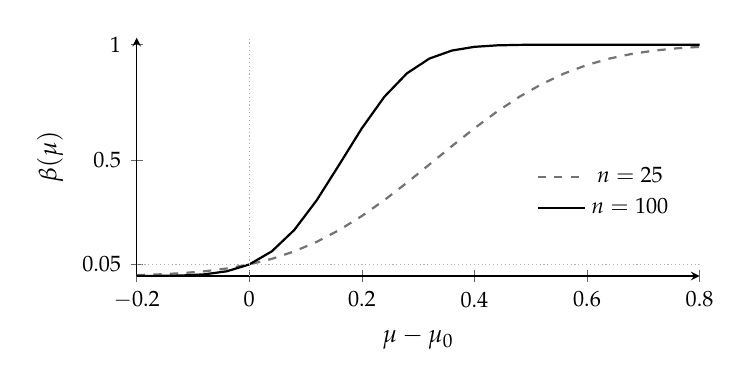
\begin{tikzpicture}
\begin{axis}[width=0.72\textwidth,height=0.38\textwidth,xmin=-0.2,xmax=0.8,ymin=0,ymax=1.03,
  xlabel={$\mu-\mu_0$},ylabel={$\beta(\mu)$},axis lines=left,tick style={black!60},
  ytick={0.05,0.5,1},yticklabels={$0.05$,$0.5$,$1$},xtick={-0.2,0,0.2,0.4,0.6,0.8},
  every axis label/.style={font=\small},ticklabel style={font=\footnotesize},
  legend style={draw=none,fill=none,font=\footnotesize,at={(0.97,0.35)},anchor=east}]
\addplot[black!55,thick,dashed] coordinates {(-0.20,0.0041) (-0.16,0.0072) (-0.12,0.0124) (-0.08,0.0204) (-0.04,0.0325) (0.00,0.0500) (0.04,0.0742) (0.08,0.1066) (0.12,0.1480) (0.16,0.1991) (0.20,0.2595) (0.24,0.3282) (0.28,0.4033) (0.32,0.4821) (0.36,0.5616) (0.40,0.6387) (0.44,0.7106) (0.48,0.7749) (0.52,0.8302) (0.56,0.8760) (0.60,0.9123) (0.64,0.9400) (0.68,0.9604) (0.72,0.9747) (0.76,0.9844) (0.80,0.9907)};
\addlegendentry{$n=25$}
\addplot[black,thick] coordinates {(-0.20,0.0001) (-0.16,0.0006) (-0.12,0.0022) (-0.08,0.0072) (-0.04,0.0204) (0.00,0.0500) (0.04,0.1066) (0.08,0.1991) (0.12,0.3282) (0.16,0.4821) (0.20,0.6387) (0.24,0.7749) (0.28,0.8760) (0.32,0.9400) (0.36,0.9747) (0.40,0.9907) (0.44,0.9971) (0.48,0.9992) (0.52,0.9998) (0.56,1.0000) (0.60,1.0000) (0.64,1.0000) (0.68,1.0000) (0.72,1.0000) (0.76,1.0000) (0.80,1.0000)};
\addlegendentry{$n=100$}
\addplot[black!30,densely dotted,domain=-0.2:0.8,samples=2] {0.05};
\addplot[black!30,densely dotted] coordinates {(0,0) (0,1.03)};
\end{axis}
\end{tikzpicture}
\caption{Power function of the one-sided 5\% test in Example~\ref{ex:onesided}. Size is controlled on the whole null $\mu\le\mu_0$ and attained at the boundary; power rises with the distance from the null and with $n$.}\label{fig:power}
\end{figure}

\subsection{Most powerful tests}

\begin{theorem}[Neyman--Pearson]\label{thm:np}
For simple $H_0:\theta=\theta_0$ against simple $H_1:\theta=\theta_1$, the test that rejects when $f(x\mid\theta_1)/f(x\mid\theta_0)>k$, with $k$ chosen so that its size is $\alpha$, is most powerful among all tests of level $\alpha$.
\end{theorem}

\begin{proof}
Let $\phi^\star=\one\{f_1>kf_0\}$ and let $\phi\in[0,1]$ be any test with $\E_0\phi\le\alpha$. Pointwise, $(\phi^\star-\phi)(f_1-kf_0)\ge0$, since $\phi^\star=1$ where $f_1-kf_0>0$ and $\phi^\star=0$ where it is negative. Integrating, $\E_1\phi^\star-\E_1\phi\ge k(\E_0\phi^\star-\E_0\phi)=k(\alpha-\E_0\phi)\ge0$.
\end{proof}

The likelihood ratio orders sample points by how much more probable they are under the alternative, and the best test rejects at the points with the highest ratio until the size budget $\alpha$ is spent. In Example~\ref{ex:onesided}, $f(x\mid\mu_1)/f(x\mid\mu_0)=\exp\{n(\mu_1-\mu_0)\bar x-\frac n2(\mu_1^2-\mu_0^2)\}$ is increasing in $\bar x$ for every $\mu_1>\mu_0$, so the same test is most powerful against every one-sided alternative: it is \emph{uniformly} most powerful. Against the two-sided alternative $\mu\ne\mu_0$ no UMP test exists, because the best test against $\mu_1>\mu_0$ rejects for large $\bar x$ and the best against $\mu_1<\mu_0$ for small $\bar x$. This is why so many tests coexist in practice, and why the large-sample tests of Section~\ref{sec:trinity} are compared through their local power.

\subsection{The $p$-value}\label{sec:pvalue}

If $H_0$ is rejected for large values of a statistic $T$, the $p$-value of the observed $t=T(x)$ is
\[
p(x)=\sup_{\theta\in\Theta_0}\P_\theta\{T(\mathcal X)\ge t\},
\]
the probability, computed under the null, of a sample at least as adverse to $H_0$ as the one observed. Rejecting when $p\le\alpha$ is the level-$\alpha$ test. Under a simple null with continuous $T$, $p=1-F_T(T)\sim U(0,1)$ by Proposition~\ref{prop:pit}, so $\P\{p\le\alpha\}=\alpha$ exactly. The $p$-value is a random variable, a function of the data. It is not the probability that $H_0$ is true (in the frequentist framework $\theta$ is not random and no such probability exists), not the probability of a false rejection (that is the size), and $1-p$ is not the probability of the alternative. Reporting $p$ lets each reader apply their own level.

\begin{example}[Testing a variance under normality]
Let $X_i\sim\N(\mu,\sigma^2)$ and $H_0:\sigma^2=\sigma_0^2$ against $H_1:\sigma^2<\sigma_0^2$, with $\mu$ unknown, so both hypotheses are composite. By Theorem~\ref{thm:gausssample}, $T=(n-1)s^2/\sigma_0^2\sim\chi^2_{n-1}$ under $H_0$ whatever $\mu$: $T$ is \emph{pivotal}. Small values favour $H_1$, so reject when $T<\chi^2_{n-1,\alpha}$. The power at $\sigma^2<\sigma_0^2$ is $F_{\chi^2_{n-1}}\big((\sigma_0^2/\sigma^2)\chi^2_{n-1,\alpha}\big)$, increasing as $\sigma^2$ falls. With $n=101$, $\sigma_0^2=1$ and $s^2=0.9$, $T=90$ and $p=F_{\chi^2_{100}}(90)\approx0.25$: a 10\% shortfall in the sample variance is well within sampling noise at this sample size.
\end{example}

\subsection{Pivots and asymptotic tests}

A statistic is \emph{pivotal} if its null distribution is free of unknown parameters, and \emph{asymptotically pivotal} if its limiting null distribution is. Pivots are what make critical values computable.

\begin{example}[The $t$-test without normality]\label{ex:ttest}
For \iid\ data with finite variance and $H_0:\mu=\mu_0$, the CLT and $s^2\cp\sigma^2$ give, by Slutsky,
\[
t=\frac{\sqrt n(\Xbar-\mu_0)}{s}\cd\N(0,1)\quad\text{under }H_0 .
\]
Rejecting when $|t|>1.96$ has asymptotic size 5\%, with $p$-value $2\Phi(-|t|)$. Under $\mu\ne\mu_0$, $t=\sqrt n(\Xbar-\mu)/s+\sqrt n(\mu-\mu_0)/s$ diverges, so the test is consistent.
\end{example}

\begin{example}[Two samples]
Let $X_1,\ldots,X_m$ and $Y_1,\ldots,Y_n$ be independent samples with means $\mu_x,\mu_y$ and variances $\sigma_x^2,\sigma_y^2$, and $H_0:\mu_x=\mu_y$. The statistic
\[
t=\frac{\bar X_m-\bar Y_n}{\sqrt{s_x^2/m+s_y^2/n}}\cd\N(0,1)\quad\text{under }H_0\text{ as }m,n\to\infty .
\]
\emph{Proof.} Let $w=(\sigma_x^2/m)/(\sigma_x^2/m+\sigma_y^2/n)\in[0,1]$, which may not converge. Under $H_0$ the numerator, divided by $(\sigma_x^2/m+\sigma_y^2/n)^{1/2}$, equals $\sqrt w\,Z_m-\sqrt{1-w}\,Z'_n$ with $Z_m=\sqrt m(\bar X_m-\mu_x)/\sigma_x$ and $Z'_n=\sqrt n(\bar Y_n-\mu_y)/\sigma_y$ independent. Its characteristic function is
\[
\varphi_{Z_m}(\sqrt w\,t)\,\varphi_{Z'_n}(-\sqrt{1-w}\,t)=e^{-wt^2/2}e^{-(1-w)t^2/2}+o(1)=e^{-t^2/2}+o(1)
\]
uniformly in $w\in[0,1]$, because characteristic functions converge uniformly on compact sets. The squared denominator, divided by the same quantity, is $w\,s_x^2/\sigma_x^2+(1-w)s_y^2/\sigma_y^2\cp1$. Slutsky completes the argument. No assumption on the relative sizes of $m$ and $n$, and no equality of variances, is needed.
\end{example}

\subsection{Bootstrap tests}\label{sec:boottest}

When the asymptotic variance is tedious to derive or poorly estimated, the bootstrap can supply critical values. To test $H_0:\V(X_i)=\sigma_0^2$ with $z=\sqrt n(s^2-\sigma_0^2)$:
\begin{itemize}
\item for $b=1,\ldots,B$, resample $\mathcal X^*_b$ from $\{X_1,\ldots,X_n\}$ with replacement, compute its sample variance $s^{*2}_b$ and $z_b^*=\sqrt n(s^{*2}_b-s^2)$;
\item accept $H_0$ if $z^*_{(\lfloor\alpha B/2\rfloor)}<z<z^*_{(\lfloor(1-\alpha/2)B\rfloor)}$, and reject otherwise.
\end{itemize}
Under $H_0$, $z\cd\N(0,\mu_4-\sigma^4)$ by Example~\ref{ex:s2}. In the bootstrap world the population variance is $s^2$ (or $\hat\sigma^2$, the difference is $O(n^{-1})$) and the fourth central moment is the consistent plug-in $\hat\mu_4$, so $z^*\cd\N(0,\hat\mu_4-\hat\sigma^4)$ conditionally, with $\hat\mu_4-\hat\sigma^4\cp\mu_4-\sigma^4$. The bootstrap quantiles therefore converge to the correct null quantiles without the variance formula ever being written down.

\begin{whybox}{the bootstrap statistic is centred at $s^2$, not at $\sigma_0^2$}
A bootstrap test must reproduce the null distribution of the test statistic \emph{whether or not $H_0$ is true}; otherwise it has no power. Centring at $s^2$ does this, because $\sqrt n(s^{*2}-s^2)$ mimics $\sqrt n(s^2-\sigma^2)$ for the true $\sigma^2$, which under $H_0$ is the law of $z$. Under the alternative, $z$ diverges while the bootstrap quantiles stay bounded, and the test rejects. Had we centred at $\sigma_0^2$, the bootstrap distribution would be located at $\sqrt n(s^2-\sigma_0^2)=z$ itself, so $z$ would always sit in the middle of its own reference distribution and the test would never reject. The general rule is ``resample in a way that respects the null'', and the simplest way to respect a null about a parameter is to centre at the estimate.
\end{whybox}

% ==================================================================
\section{Large-sample tests: the likelihood trinity}\label{sec:trinity}
% ==================================================================

Let $X_i$ be \iid\ $f(\cdot\mid\theta)$ under the MLE regularity conditions, $\theta\in\R^k$, and $H_0:g(\theta)=0$ with $g:\R^k\to\R^p$ smooth and $G(\theta)=\partial g/\partial\theta^\top$ of rank $p$. Let $\thml$ be the unrestricted MLE and $\hat\theta_0=\argmax_{g(\theta)=0}\ell(\theta)$ the restricted one. Three statistics look at the log-likelihood from three different places.

\subsection{Likelihood ratio}

\begin{theorem}\label{thm:lr}
For scalar $\theta$ and $H_0:\theta=\theta_0$, $LR=-2\log\{L(\theta_0)/L(\thml)\}=2\{\ell(\thml)-\ell(\theta_0)\}\cd\chi^2_1$. In general, $LR=2\{\ell(\thml)-\ell(\hat\theta_0)\}\cd\chi^2_p$ under $H_0$.
\end{theorem}

\begin{proof}[Proof \textup{(}scalar case\textup{)}]
Expand around $\thml$, where the score vanishes: for $\theta^\star$ between $\theta_0$ and $\thml$,
\[
LR=-2\Big[S(\thml)(\theta_0-\thml)+\tfrac12\partial_\theta S(\theta^\star)(\theta_0-\thml)^2\Big]=\Big[-\tfrac1n\partial_\theta S(\theta^\star)\Big]\cdot n(\thml-\theta_0)^2 .
\]
The bracket converges in probability to $I_1(\theta_0)$ (as in Theorem~\ref{thm:mlean}), and $\sqrt n(\thml-\theta_0)\cd\N(0,I_1^{-1})$, so $LR=I_1\cdot\{\N(0,I_1^{-1})\}^2+\op(1)\cd\chi^2_1$.
\end{proof}

\subsection{Wald}

Suppose $\sqrt n(\hat\theta-\theta)\cd\N(0,V)$ and $\hat V\cp V$. The delta method gives
\[
\sqrt n\{g(\hat\theta)-g(\theta)\}\cd\N(0,GVG^\top),
\]
and under $H_0$
\[
W=n\,g(\hat\theta)^\top\big[\hat G\hat V\hat G^\top\big]^{-1}g(\hat\theta)\cd\chi^2_p,\qquad\hat G=G(\hat\theta),
\]
because $(GVG^\top)^{-1/2}\sqrt n\,g(\hat\theta)\cd\N(0,I_p)$ and the squared norm of a standard normal $p$-vector is $\chi^2_p$. For the MLE, $V=I_1^{-1}$; for scalar $H_0:\theta=\theta_0$, $W=nI_1(\thml)(\thml-\theta_0)^2$. The Wald test needs only the unrestricted estimate.

\subsection{Score (Lagrange multiplier)}

The first information equality says $\E_{\theta_0}S(\theta_0)=0$. The score test checks whether this moment condition holds at the hypothesised value. Under $H_0$, $n^{-1/2}S(\theta_0)\cd\N(0,I_1(\theta_0))$ by the CLT, so
\[
LM=\frac{S(\theta_0)^2}{nI_1(\theta_0)}\cd\chi^2_1,\qquad LM=\frac1nS(\hat\theta_0)^\top I_1(\hat\theta_0)^{-1}S(\hat\theta_0)\cd\chi^2_p\ \text{in general}.
\]
The name comes from the constrained problem $\max\ell(\theta)$ s.t.\ $\theta=\theta_0$: the Lagrangian $\ell(\theta)-\lambda(\theta-\theta_0)$ has first-order condition $\lambda=S(\theta_0)$, so the score measures the shadow value of the restriction, how much the likelihood wants to move away from it. The LM test needs only the restricted estimate.

\subsection{Equivalence, geometry, and differences}

All three are quadratic approximations to the same object. Expanding $S(\theta_0)=S(\theta_0)-S(\thml)=\partial_\theta S(\theta^\star)(\theta_0-\thml)$,
\[
LM=\frac{\{-n^{-1}\partial_\theta S(\theta^\star)\}^2}{I_1(\theta_0)}\,n(\thml-\theta_0)^2=nI_1(\theta_0)(\thml-\theta_0)^2\{1+\op(1)\},
\]
and $W$ and $LR$ have the same leading term. Hence $LR-W\cp0$ and $LM-LR\cp0$ under $H_0$ (and under local alternatives): the three tests are asymptotically equivalent. Figure~\ref{fig:trinity} shows what each measures.

\begin{figure}[h]
\centering
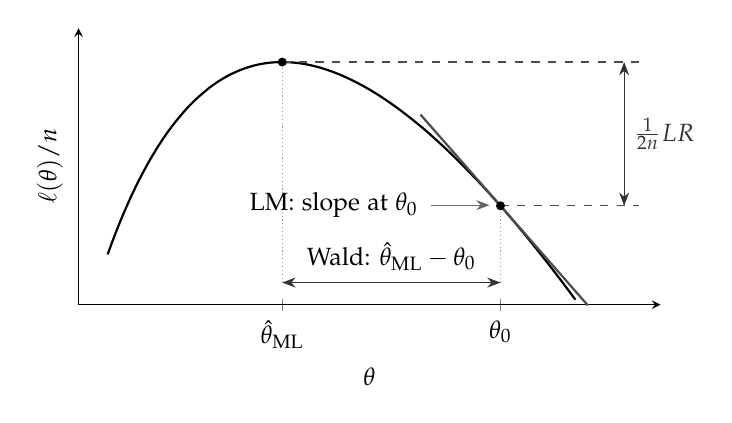
\begin{tikzpicture}[>=Stealth]
\begin{axis}[width=0.74\textwidth,height=0.42\textwidth,xmin=2.2,xmax=10.2,ymin=1.95,ymax=3.2,
  axis lines=left,xlabel={$\theta$},ylabel={$\ell(\theta)/n$},xtick={5,8},xticklabels={$\thml$,$\theta_0$},
  ytick=\empty,every axis label/.style={font=\small},ticklabel style={font=\small},clip=false]
\addplot[black,thick,domain=2.6:9.03,samples=120] {5*ln(x)-x+0.0};
% points
\addplot[only marks,mark=*,mark size=1.4pt] coordinates {(5,{5*ln(5)-5}) (8,{5*ln(8)-8})};
% LR vertical gap
\draw[black!70,dashed] (axis cs:5,{5*ln(5)-5}) -- (axis cs:9.9,{5*ln(5)-5});
\draw[<->,black!80] (axis cs:9.7,{5*ln(5)-5}) -- node[right,font=\small]{$\tfrac{1}{2n}LR$} (axis cs:9.7,{5*ln(8)-8});
\draw[black!70,dashed] (axis cs:8,{5*ln(8)-8}) -- (axis cs:9.9,{5*ln(8)-8});
% Wald horizontal
\draw[<->,black!80] (axis cs:5,2.05) -- (axis cs:8,2.05); \node[font=\small,above] at (axis cs:6.5,2.06) {Wald: $\thml-\theta_0$};
\draw[black!40,densely dotted] (axis cs:5,2.05) -- (axis cs:5,{5*ln(5)-5});
\draw[black!40,densely dotted] (axis cs:8,2.05) -- (axis cs:8,{5*ln(8)-8});
% LM tangent at theta0: slope 5/8-1=-0.375
\draw[black!70,thick] (axis cs:6.9,{5*ln(8)-8+0.4125}) -- (axis cs:9.2,{5*ln(8)-8-0.45});
\node[font=\small,anchor=east] at (axis cs:7.0,2.40) {LM: slope at $\theta_0$}; \draw[->,black!60] (axis cs:7.05,2.40) -- (axis cs:7.85,2.40);
\end{axis}
\end{tikzpicture}
\caption{The trinity on the Poisson log-likelihood $\ell(\lambda)/n=\bar x\log\lambda-\lambda$ (up to a constant) with $\bar x=5$. Wald measures the horizontal distance between the estimate and the null, weighted by the curvature at $\thml$; LR measures the vertical drop in the log-likelihood; LM measures the slope at the null, weighted by the curvature at $\theta_0$. For a quadratic log-likelihood the three coincide.}\label{fig:trinity}
\end{figure}

\begin{example}[Poisson]\label{ex:poisson}
Let $X_i\sim$ Poisson$(\lambda)$, $H_0:\lambda=\lambda_0=6$, with $n=100$ and $\Xbar=5$. Then $\ell(\lambda)=\sum x_i\log\lambda-n\lambda-\sum\log x_i!$, $S(\lambda)=\sum x_i/\lambda-n$, $\hat\lambda=\Xbar$, and $I_1(\lambda)=-\E\partial^2_\lambda\ell_1=\E X/\lambda^2=1/\lambda$.
\[
\begin{aligned}
LR&=2n\big[\Xbar\log(\Xbar/\lambda_0)-\Xbar+\lambda_0\big]=200\,[5\log(5/6)+1]\approx17.68,\\
W&=nI_1(\hat\lambda)(\hat\lambda-\lambda_0)^2=100\cdot(5-6)^2/5=20.00,\\
LM&=\frac{S(\lambda_0)^2}{nI_1(\lambda_0)}=\frac{(500/6-100)^2}{100/6}=\frac{n(\Xbar-\lambda_0)^2}{\lambda_0}\approx16.67 .
\end{aligned}
\]
All exceed $\chi^2_{1,0.95}=3.84$, with $p$-values from about $8\times10^{-6}$ (Wald) to $4.5\times10^{-5}$ (LM). Here $LM<LR<W$. That ordering is a theorem in the Gaussian linear regression model (Berndt and Savin, 1977), but not in general: $W$ and $LM$ differ only in whether the variance $\lambda$ is evaluated at $\hat\lambda$ or at $\lambda_0$, so with $\Xbar=7$ the ordering of $W$ and $LM$ would reverse.
\end{example}

\paragraph{Invariance}
$LR$ and $LM$ depend on the null only through the restricted set $\Theta_0$, so any reformulation $g\mapsto h\circ g$ with $h$ invertible, $h(0)=0$, leaves them unchanged. The Wald statistic is not invariant. With $X_i\sim\N(\mu,\sigma^2)$, $\sigma$ known, the null $\mu=0$ gives $W_1=n\Xbar^2/\sigma^2$. Writing the same null as $\mu^3=0$, the delta-method variance is $(3\Xbar^2)^2\sigma^2$, and
\[
W_3=\frac{n\Xbar^6}{9\Xbar^4\sigma^2}=\frac{W_1}{9}.
\]
A sample with $W_1=9$ ($p\approx0.003$) gives $W_3=1$ ($p\approx0.32$). The source is the rank condition: $G(\mu)=3\mu^2$ vanishes at the null, the delta method degenerates, and $W_3\cd\chi^2_1/9$ under $H_0$, so the test based on $\chi^2_1$ critical values almost never rejects. Less extreme versions of the problem afflict every nonlinear restriction; the remedy is to write the restriction in a form that is as close to linear as possible, or to use LR or LM.

\begin{table}[h]
\centering\small
\caption{The trinity at a glance}\label{tab:trinity}
\begin{tabular}{@{}lllll@{}}
\toprule
Test & Statistic & Requires & Invariant & Geometry\\
\midrule
LR & $2\{\ell(\thml)-\ell(\hat\theta_0)\}$ & both estimates & yes & height\\
Wald & $n\,g(\thml)^\top\hat\Sigma^{-1}g(\thml)$ & $\thml$ and $\hat I$ & no & horizontal distance\\
LM & $n^{-1}S(\hat\theta_0)^\top I_1(\hat\theta_0)^{-1}S(\hat\theta_0)$ & $\hat\theta_0$ and $I_1$ & yes & slope\\
\bottomrule
\end{tabular}
\end{table}

\begin{whybox}{three tests rather than one}
They answer the same question at different computational costs. Wald is convenient when the unrestricted model is easy to estimate and the restrictions are linear. LM is convenient when the restricted model is easy and the unrestricted one hard, as in specification tests where the null is the simple model and the alternative a complicated generalisation. LR requires both, but it is invariant and, in finite samples, typically has the most reliable size. Asymptotically they are identical; their finite-sample differences are a symptom of how far the log-likelihood is from quadratic.
\end{whybox}

% ==================================================================
\section{Confidence sets}\label{sec:ci}
% ==================================================================

\subsection{Coverage and test inversion}

A confidence set $C(\mathcal X)\subset\Theta$ is a random set. Its coverage at $\theta$ is $\P_\theta\{\theta\in C(\mathcal X)\}$, and it has confidence level $1-\alpha$ if $\inf_{\theta\in\Theta}\P_\theta\{\theta\in C(\mathcal X)\}\ge1-\alpha$. The randomness is in the set, not in $\theta$: ``95\%'' describes the procedure across repeated samples, not the realised interval.

\begin{theorem}[Test inversion]\label{thm:inversion}
Suppose that for each $\theta_0\in\Theta$ there is a test of $H_0:\theta=\theta_0$ of level $\alpha$. Then $C(\mathcal X)=\{\theta_0:\text{the test of }\theta=\theta_0\text{ accepts}\}$ has confidence level $1-\alpha$. Conversely, a level-$(1-\alpha)$ confidence set yields a level-$\alpha$ test that accepts $\theta=\theta_0$ iff $\theta_0\in C(\mathcal X)$.
\end{theorem}

\begin{proof}
If the truth is $\theta_0$, then $\theta_0\notin C(\mathcal X)$ exactly when the test of $\theta_0$ rejects, which has probability at most $\alpha$. This holds for every $\theta_0$.
\end{proof}

\begin{example}[Mean]
Inverting the asymptotic $t$-test of Example~\ref{ex:ttest}, $\theta_0$ is accepted iff $z_{\alpha/2}\le\sqrt n(\Xbar-\mu_0)/s\le z_{1-\alpha/2}$, i.e.
\[
\mu_0\in\Big[\Xbar-z_{1-\alpha/2}\frac{s}{\sqrt n},\;\Xbar-z_{\alpha/2}\frac{s}{\sqrt n}\Big]=\Xbar\pm z_{1-\alpha/2}\frac{s}{\sqrt n},
\]
an interval of asymptotic level $1-\alpha$ whose half-width is a multiple of the standard error $s/\sqrt n$.
\end{example}

\paragraph{Wald intervals for a function of $\theta$}
For $\tau=h(\theta)$ with $h'(\theta)\ne0$, the delta method gives $\sqrt n\{h(\thml)-h(\theta)\}\cd\N(0,h'(\theta)^2I_1^{-1})$. With $\hat V=h'(\thml)^2\{-\partial^2_\theta\ell(\thml)\}^{-1}$, which already includes the factor $1/n$, inversion gives
\[
\Big[h(\thml)-z_{1-\alpha/2}\hat V^{1/2},\;h(\thml)+z_{1-\alpha/2}\hat V^{1/2}\Big].
\]

\begin{example}[Odds]
For Bernoulli data and $h(p)=p/(1-p)$, $h'(p)=1/(1-p)^2$, so $\sqrt n\{h(\hat p)-h(p)\}\cd\N\big(0,p/(1-p)^3\big)$ and $\hat V=\hat p/\{(1-\hat p)^3n\}$. With $n=100$ and $\hat p=0.2$, the odds estimate is $0.25$ with standard error $0.0625$, and the 95\% interval is $[0.128,\,0.372]$. Because the odds are a monotone function of $p$, an alternative is to map an interval for $p$ through $h$; coverage is preserved exactly, and the result is not symmetric around $0.25$. The choice matters in small samples or when $p$ is near $0$ or $1$: Wald intervals are symmetric by construction and can extend outside the parameter space, while inverting the score test (the Wilson interval for $p$) does not.
\end{example}

\paragraph{Optimality}
Pratt's theorem connects the length of a confidence set to the power of the tests it inverts. By Fubini,
\[
\E_{\theta_0}\big[\text{length of }C(\mathcal X)\big]=\E_{\theta_0}\int\one\{\theta\in C(\mathcal X)\}\,d\theta=\int\P_{\theta_0}\{\theta\in C(\mathcal X)\}\,d\theta .
\]
The integrand at $\theta\ne\theta_0$ is the probability of accepting the false value $\theta$, one minus the power of the test of $\theta$ against $\theta_0$. Inverting uniformly most powerful tests therefore minimises the integrand pointwise and gives the shortest expected length among all sets of level $1-\alpha$. Short intervals are powerful tests in disguise.

\subsection{Bootstrap confidence sets}\label{sec:bootci}

Let $\hat\theta=\delta(\mathcal X)$ be consistent. To test $\theta=\theta_0$, use $T(\theta_0)=\hat\theta-\theta_0$ and approximate its null law by that of $T^*=\delta(\mathcal X^*)-\hat\theta$ under resampling from $\hat F$:
\begin{itemize}
\item for $b=1,\ldots,B$, draw $\mathcal X^*_b$ from $\hat F$ and compute $T_b^*=\delta(\mathcal X_b^*)-\hat\theta$; order them as $T^*_{(1)}\le\dots\le T^*_{(B)}$;
\item accept $\theta=\theta_0$ iff $T^*_{(\lfloor\alpha B/2\rfloor)}\le\hat\theta-\theta_0\le T^*_{(\lfloor(1-\alpha/2)B\rfloor)}$;
\item invert: $C=\big[\hat\theta-T^*_{(\lfloor(1-\alpha/2)B\rfloor)},\;\hat\theta-T^*_{(\lfloor\alpha B/2\rfloor)}\big]$.
\end{itemize}

\begin{whybox}{the quantiles appear reversed}
The interval is a statement about where $\theta$ lies given $\hat\theta$, but the bootstrap estimates the law of the error $\hat\theta-\theta$. If the error is skewed to the right (large positive errors are common), then a high value of $\hat\theta$ is more likely due to overshooting, and the interval must extend further \emph{below} $\hat\theta$: the upper error quantile sets the lower endpoint. This is also why the interval ``implicitly bias-corrects'': if the bootstrap errors are centred at a positive value, the whole interval shifts down. The naive percentile interval $[\hat\theta^*_{(\alpha/2)},\hat\theta^*_{(1-\alpha/2)}]$ coincides with this basic interval only when the error distribution is symmetric. Bootstrapping the studentised statistic $(\delta(\mathcal X^*)-\hat\theta)/\mathrm{se}^*$ instead yields $[\hat\theta-Z^*_{(1-\alpha/2)}\mathrm{se},\,\hat\theta-Z^*_{(\alpha/2)}\mathrm{se}]$; because the studentised statistic is asymptotically pivotal, its bootstrap approximation is accurate to a higher order, and the coverage error typically falls from $O(n^{-1/2})$ to $O(n^{-1})$ for one-sided intervals (Hall, 1992). All of these intervals inherit the failures of Example~\ref{ex:bootmax}: they need a smooth problem.
\end{whybox}

% ==================================================================
\section{The Bayesian paradigm}\label{sec:bayes}
% ==================================================================

\subsection{Two views of uncertainty}

In the frequentist paradigm used so far, $\theta$ is fixed and unknown, the data are random, and every guarantee (unbiasedness, size, coverage) is a statement about the distribution of a procedure across hypothetical repeated samples. In the Bayesian paradigm, $\theta$ is itself random with a \emph{prior} density $\pi(\theta)$ expressing what is believed before seeing the data. Given $\theta$, the data are drawn from $f(x\mid\theta)$, so the joint density is $\pi(\theta)f(x\mid\theta)$. Once $x$ is observed it is treated as fixed, and all uncertainty is about $\theta$, summarised by the \emph{posterior}
\[
\pi(\theta\mid x)=\frac{\pi(\theta)f(x\mid\theta)}{m(x)},\qquad m(x)=\int\pi(\tilde\theta)f(x\mid\tilde\theta)\,d\tilde\theta,
\]
which is Bayes' rule \eqref{eq:bayes} for densities. The marginal $m(x)$, the prior predictive density of the data, does not depend on $\theta$, so in practice one computes $\pi(\theta\mid x)\propto\pi(\theta)f(x\mid\theta)$ and normalises at the end.

\subsection{Conjugate families}\label{sec:conj}

A family of priors is \emph{conjugate} to a model if the posterior stays in the family. Conjugacy turns updating into arithmetic on parameters.

\begin{example}[Normal mean with a normal prior]\label{ex:normalprior}
Let $X_i\sim\N(\mu,\sigma^2)$ with $\sigma^2$ known and prior $\mu\sim\N(\mu_0,\tau^2)$. Keeping only terms that involve $\mu$,
\[
\pi(\mu\mid x)\propto\exp\Big\{-\frac{\sum_i(x_i-\mu)^2}{2\sigma^2}-\frac{(\mu-\mu_0)^2}{2\tau^2}\Big\}
\propto\exp\Big\{-\frac12\Big(\frac{n}{\sigma^2}+\frac1{\tau^2}\Big)\mu^2+\Big(\frac{n\bar x}{\sigma^2}+\frac{\mu_0}{\tau^2}\Big)\mu\Big\}.
\]
Completing the square, $\mu\mid x\sim\N(\tilde\mu,\tilde\sigma^2)$ with
\[
\frac1{\tilde\sigma^2}=\frac{n}{\sigma^2}+\frac1{\tau^2},\qquad
\tilde\mu=\frac{(n/\sigma^2)\,\bar x+(1/\tau^2)\,\mu_0}{n/\sigma^2+1/\tau^2}.
\]
\end{example}

\begin{whybox}{the posterior mean is a shrinkage estimator}
Precisions add: the posterior precision is the data precision $n/\sigma^2$ plus the prior precision $1/\tau^2$. The posterior mean is the precision-weighted average of the sample mean and the prior mean,
\[
\tilde\mu=(1-c)\,\bar x+c\,\mu_0,\qquad c=\frac{1/\tau^2}{n/\sigma^2+1/\tau^2}=\frac{\sigma^2}{\sigma^2+n\tau^2},
\]
which is exactly the shrinkage estimator of Section~\ref{sec:finite}, with the amount of shrinkage determined by how much the prior is trusted relative to the data. A tight prior ($\tau^2$ small) pulls the estimate to $\mu_0$; a diffuse prior ($\tau^2\to\infty$) gives $c\to0$ and $\tilde\mu\to\bar x$. As $n\to\infty$, $c\to0$ and $\tilde\sigma^2\to0$: the data swamp the prior and the posterior concentrates at the truth. From the frequentist side, $\tilde\mu$ is biased toward $\mu_0$ but has smaller variance than $\bar x$, and it has smaller MSE whenever $\mu$ is close enough to $\mu_0$. The Bayesian prior is one principled way to choose the shrinkage point and amount.
\end{whybox}

\begin{example}[Bernoulli with a uniform prior]
Let $X_i\sim$ Bernoulli$(p)$ and $\pi(p)=\one\{p\in[0,1]\}$. With $t=\sum_ix_i$,
\[
\pi(p\mid x)\propto p^{t}(1-p)^{n-t},
\]
the kernel of a Beta$(t+1,n-t+1)$ density. More generally a Beta$(a,b)$ prior gives a Beta$(a+t,\,b+n-t)$ posterior: the prior acts like $a$ prior successes and $b$ prior failures. Under the uniform prior the posterior mean is $(t+1)/(n+2)$, Laplace's rule of succession, which shrinks $\hat p=t/n$ toward $\frac12$. After $n=10$ flips with no heads, the MLE says $p=0$ while the posterior mean is $1/12$: the prior prevents the estimate from asserting impossibility on the basis of a small sample.
\end{example}

\subsection{Bayesian estimation, intervals and tests}

A point estimate minimises posterior expected loss. Under squared loss, $\E[(\theta-a)^2\mid x]=\V(\theta\mid x)+(\E[\theta\mid x]-a)^2$ is minimised at the posterior mean; under absolute loss, at the posterior median; the posterior mode is the limit under 0--1 loss.

A set $C(x)$ is $(1-\alpha)$-\emph{credible} if $\pi\{\theta\in C(x)\mid x\}\ge1-\alpha$. The shortest such set collects the points of highest posterior density. In Example~\ref{ex:normalprior}, $[\tilde\mu\pm z_{1-\alpha/2}\tilde\sigma]$ is the shortest credible interval, by the symmetry and unimodality of the normal density. As $\tau^2\to\infty$ it becomes $\bar x\pm z_{1-\alpha/2}\sigma/\sqrt n$, numerically the frequentist confidence interval. The interpretations remain different: the credible statement is a probability about $\theta$ given the realised data; the confidence statement is a probability about the interval across samples.

To test $H_0:\theta\in\Theta_0$ against $H_1:\theta\in\Theta_1$, the Bayesian compares posterior probabilities, accepting $H_0$ iff $\pi(\Theta_0\mid x)\ge\pi(\Theta_1\mid x)$. The hypotheses are treated symmetrically, unlike in the Neyman--Pearson framework. A point null $\theta=\theta_0$ has zero posterior probability under a continuous prior, so testing it requires a prior that puts positive mass on $\theta_0$.

\begin{whybox}{the two paradigms agree in large samples, and where they do not}
Under the regularity conditions of Theorem~\ref{thm:mlean} and a prior that is continuous and positive at $\theta_0$, the Bernstein--von Mises theorem states that the posterior is asymptotically $\N\big(\thml,\{nI_1(\theta_0)\}^{-1}\big)$: the prior washes out, the posterior mean and the MLE differ by $\op(n^{-1/2})$, and credible intervals become asymptotically valid confidence intervals. The agreement fails exactly where the frequentist theory fails, at boundaries, in irregular models and with many parameters; and it fails whenever the prior excludes the truth. If $\pi(\theta_0)=0$ on a neighbourhood of $\theta_0$, no amount of data moves posterior mass there, because the posterior is proportional to the prior. In small samples the prior matters, which is a cost when it is arbitrary and a benefit when it encodes real information, as with shrinkage across many related parameters.
\end{whybox}

% ==================================================================
\section*{Synthesis}
\addcontentsline{toc}{section}{Synthesis}
\markboth{Synthesis}{}
% ==================================================================

Four ideas organise the week.

The first is the \emph{analogy principle}. A parameter is defined by a population problem (a mean minimises squared error, a pseudo-true value minimises Kullback--Leibler divergence, a moment condition holds at the truth), and the estimator solves the sample version. The plug-in estimator $T(\Fn)$, the method of moments, and maximum likelihood, the method of moments for the score, are three expressions of this principle, and the bootstrap applies it to the whole sampling distribution. Its validity rests on the empirical distribution approximating the population at the scale that matters, which is why it succeeds for the mean and fails for the maximum.

The second is \emph{reduction to averages}. Every asymptotic result in these notes, from the delta method to the MLE, the trinity and the bootstrap, is proved by writing the object of interest as a smooth function of averages, applying the LLN to the parts that settle and the CLT to the part that fluctuates, and combining them with Slutsky's lemma. Rates other than $\sqrt n$ and limits other than the normal appear exactly when this reduction breaks: zero derivatives, moving supports, boundaries, and growing numbers of parameters.

The third is \emph{information}. The curvature of the log-likelihood, the Fisher information, bounds the precision of unbiased estimators, is attained asymptotically by maximum likelihood, and calibrates all three large-sample tests. Efficiency and power are the same thing seen from two sides: an estimator with half the variance supports tests that detect alternatives $\sqrt2$ times closer, and inverting the most powerful tests yields the shortest confidence sets.

The fourth is the \emph{bias--variance trade-off}. Unbiasedness is neither necessary nor sufficient for a good estimator: dividing a sum of squares by $n+1$ beats dividing by $n-1$, shrinkage improves on unbiased estimators locally and, in several dimensions, globally, and the Bayesian posterior mean is a shrinkage estimator whose amount of shrinkage is set by the prior. Much of modern econometrics, from ridge regression to empirical Bayes to regularised machine learning, elaborates this one observation.

% ==================================================================
\section*{References}
\addcontentsline{toc}{section}{References}
\markboth{References}{}
% ==================================================================
{\small
\setstretch{1.05}
\begin{description}[leftmargin=1.4em,labelindent=0pt,itemsep=2pt,font=\normalfont]
\item Berndt, E.~R.\ and N.~E.~Savin (1977). Conflict among criteria for testing hypotheses in the multivariate linear regression model. \emph{Econometrica} 45, 1263--1277.
\item Billingsley, P. (1995). \emph{Probability and Measure}, 3rd ed. Wiley.
\item Casella, G.\ and R.~L.~Berger (2002). \emph{Statistical Inference}, 2nd ed. Duxbury.
\item Efron, B.\ and R.~J.~Tibshirani (1993). \emph{An Introduction to the Bootstrap}. Chapman \& Hall.
\item Hall, P. (1992). \emph{The Bootstrap and Edgeworth Expansion}. Springer.
\item Hansen, B.~E. (2022). \emph{Probability and Statistics for Economists}. Princeton University Press.
\item Hogg, R.~V., J.~W.~McKean and A.~T.~Craig (2019). \emph{Introduction to Mathematical Statistics}, 8th ed. Pearson.
\item Lehmann, E.~L.\ and G.~Casella (1998). \emph{Theory of Point Estimation}, 2nd ed. Springer.
\item Lehmann, E.~L.\ and J.~P.~Romano (2005). \emph{Testing Statistical Hypotheses}, 3rd ed. Springer.
\item Mikusheva, A. Lecture notes 1--10, Swiss Program for Beginning Doctoral Students in Economics, Study Center Gerzensee.
\item Neyman, J.\ and E.~L.~Scott (1948). Consistent estimates based on partially consistent observations. \emph{Econometrica} 16, 1--32.
\item Stein, C. (1956). Inadmissibility of the usual estimator for the mean of a multivariate normal distribution. \emph{Proceedings of the Third Berkeley Symposium} 1, 197--206.
\item van der Vaart, A.~W. (1998). \emph{Asymptotic Statistics}. Cambridge University Press.
\end{description}
}


\end{document}
